% Copyright 2004 by Till Tantau <tantau@users.sourceforge.net>.
%
% In principle, this file can be redistributed and/or modified under
% the terms of the GNU Public License, version 2.
%
% However, this file is supposed to be a template to be modified
% for your own needs. For this reason, if you use this file as a
% template and not specifically distribute it as part of a another
% package/program, I grant the extra permission to freely copy and
% modify this file as you see fit and even to delete this copyright
% notice. 

\documentclass[aspectratio=169]{beamer}
%\documentclass{beamer}

\setbeamersize{text margin left=5mm, text margin right=5mm}


\defbeamertemplate{headline}{my header}{%
\vskip1pt%
\makebox[0pt][l]{\,\insertshortauthor}%
\hspace*{\fill}\insertshorttitle/\insertshortsubtitle\hspace*{\fill}%
\llap{\insertpagenumber/\insertpresentationendpage\,}
}
\setbeamertemplate{headline}[my header]

\let\olditem\item
\renewcommand{\item}{\setlength{\itemsep}{\fill}\olditem}

\usepackage{soul}
\usepackage{tkz-euclide}
\usetikzlibrary{calc}
\usepackage[]{algorithm2e}
\usepackage{changepage}
\usepackage{amssymb}
\usepackage{xcolor}
\usepackage{mathtools}
\usepackage{tcolorbox}
\usepackage{tikz}
\usepackage{tikz-3dplot}

% \usepackage[math]{cellspace}
% \cellspacetoplimit 4pt
% \cellspacebottomlimit 4pt
%\usetikzlibrary{arrows.meta}

%\setbeamertemplate{itemize items}{-}

%\usepackage{helvet}
\usefonttheme{professionalfonts} % using non standard fonts for beamer
%\usefonttheme{serif} % default family is serif
%\usepackage{fontspec}
%\setmainfont{Liberation Serif}

% There are many different themes available for Beamer. A comprehensive
% list with examples is given here:
% http://deic.uab.es/~iblanes/beamer_gallery/index_by_theme.html
% You can uncomment the themes below if you would like to use a different
% one:
%\usetheme{AnnArbor}
%\usetheme{Antibes}
%\usetheme{Bergen}
%\usetheme{Berkeley}
%\usetheme{Berlin}
%\usetheme{Boadilla}
%\usetheme{boxes}
%\usetheme{CambridgeUS}
%\usetheme{Copenhagen}
%\usetheme{Darmstadt}
%\usetheme{default}
%\usetheme{Frankfurt}
%\usetheme{Goettingen}
%\usetheme{Hannover}
%\usetheme{Ilmenau}
%\usetheme{JuanLesPins}
%\usetheme{Luebeck}
%\usetheme{Madrid}
%\usetheme{Malmoe}
%\usetheme{Marburg}
%\usetheme{Montpellier}
%\usetheme{PaloAlto}
%\usetheme{Pittsburgh}
%\usetheme{Rochester}
%\usetheme{Singapore}
%\usetheme{Szeged}
%\usetheme{Warsaw}


\def\mf{\ensuremath\mathbf}
\def\mb{\ensuremath\mathbb}
\def\lp{\ensuremath\left(}
\def\rp{\ensuremath\right)}
\def\lv{\ensuremath\left\lvert}
\def\rv{\ensuremath\right\rvert}
\def\lV{\ensuremath\left\lVert}
\def\rV{\ensuremath\right\rVert}
\def\lc{\ensuremath\left\{}
\def\rc{\ensuremath\right\}}
\def\ls{\ensuremath\left[}
\def\rs{\ensuremath\right]}
\def\bmx{\ensuremath\begin{bmatrix*}[r]}
\def\emx{\ensuremath\end{bmatrix*}}
\def\bmxc{\ensuremath\begin{bmatrix*}[c]}
\def\t{\lp t\rp}
\def\k{\ls k\rs}


\newcommand{\demoex}[2]{\onslide<#1->\begin{color}{black!60} #2 \end{color}}
\newcommand{\demoexc}[3]{\onslide<#1->\begin{color}{#2} #3 \end{color}}
\newcommand{\anim}[3]{\onslide<#1->{\begin{color}{#2!60} #3 \end{color}}}
\newcommand{\ct}[1]{\lp #1\rp}
\newcommand{\dt}[1]{\ls #1\rs}
\newcommand{\cols}[2]{\begin{columns}[#1] #2 \end{columns}}
\newcommand{\col}[2]{\begin{column}{#1} #2 \end{column}}


\title{Introduction to Digital Signal Processing}

% A subtitle is optional and this may be deleted
\subtitle{Geometric Signal Theory}

\author{Sivakumar Balasubramanian}
% - Give the names in the same order as the appear in the paper.
% - Use the \inst{?} command only if the authors have different
%   affiliation.

\institute[Christian Medical College] % (optional, but mostly needed)
{
  \inst{}%
  Department of Bioengineering\\
  Christian Medical College, Bagayam\\
  Vellore 632002
}
% - Use the \inst command only if there are several affiliations.
% - Keep it simple, no one is interested in your street address.

\date{}
% - Either use conference name or its abbreviation.
% - Not really informative to the audience, more for people (including
%   yourself) who are reading the slides online

\subject{Lecture slides on Introduction to DSP}
% This is only inserted into the PDF information catalog. Can be left
% out. 

% If you have a file called "university-logo-filename.xxx", where xxx
% is a graphic format that can be processed by latex or pdflatex,
% resp., then you can add a logo as follows:

% \pgfdeclareimage[height=0.5cm]{university-logo}{university-logo-filename}
% \logo{\pgfuseimage{university-logo}}

% Delete this, if you do not want the table of contents to pop up at
% the beginning of each subsection:
\AtBeginSubsection[]
{
  \begin{frame}<beamer>{Outline}
    \tableofcontents[currentsection,currentsubsection]
  \end{frame}
}

% Let's get started
\begin{document}

\begin{frame}
  \titlepage
\end{frame}

\begin{frame}{Geometric Signal Theory}
\begin{itemize}
  \item An interesting viewpoint that can help understand signal processing.
  \item Provide a geometric view of signals and some important signal processing operations.
\end{itemize}
\end{frame}

\begin{frame}[t]{Discrete-time Signals as Vector}

All practical signals we deal with are of finite duration.

Consider two finite duration real discrete-time signal 
\[ x[n] = \lp x_0, x_1 \rp = \bmx x_0 & x_1\emx^\top  \quad \quad y[n] = \lp y_0, y_1 \rp = \bmx y_0 & y_1 \emx^\top, \,\, n \in \{0, 1\} \]

\begin{figure}
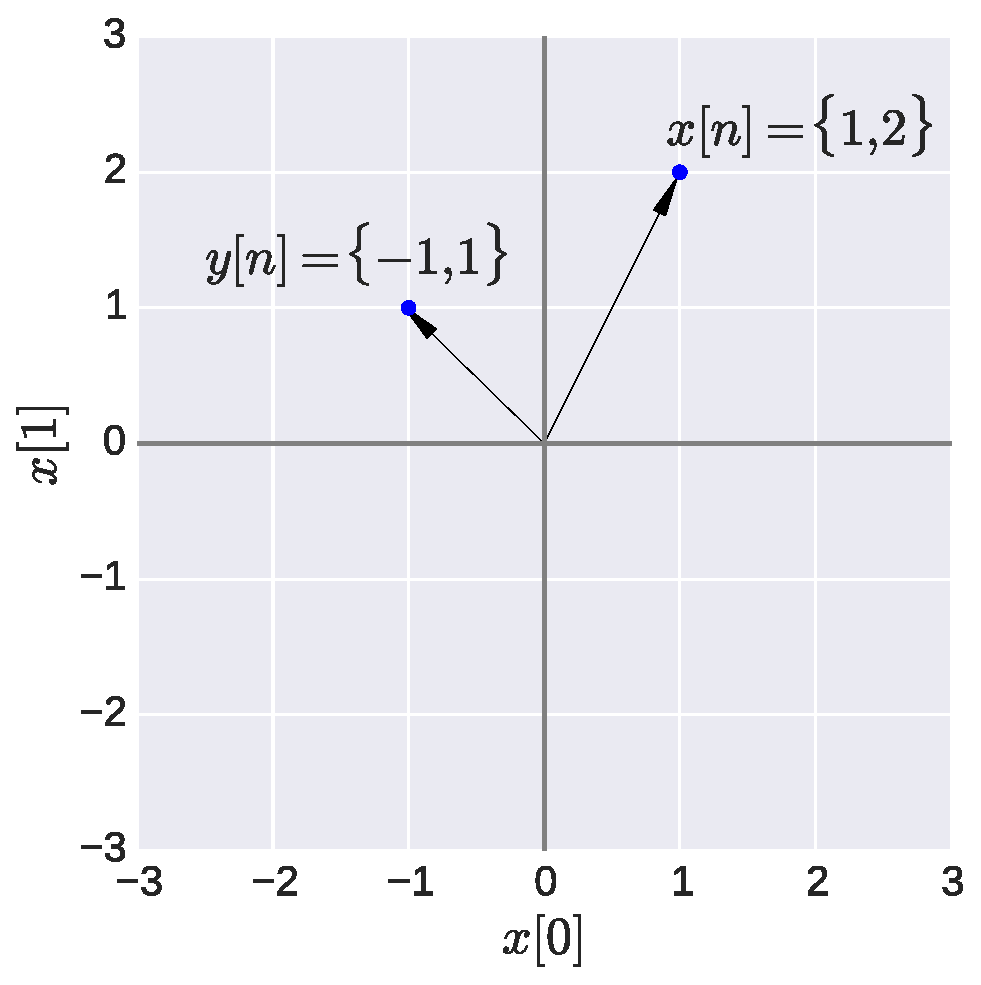
\includegraphics[width=0.35\textwidth]{img/2dvec.eps}
\end{figure}

\end{frame}

% SOME FAMILIAR GEOMETRICAL IDEAS
\begin{frame}[t]{Some familiar and useful geometric ideas}

\begin{itemize}
\item \textbf{Length} of a vector.
\[ \|x\| = \sqrt{x_0^2 + x_1^2} = \sqrt{\text{Energy of the signal}} \]
\item \textbf{Distance} between vectors.
\[ \|x - y\| = \sqrt{\left(x_0 - y_0\right)^2 + \left(x_1 - y_1\right)^2} \]
\item \textbf{Scalar product} or \textbf{Inner product} between vectors.
\[ \langle x, y \rangle = x_0y_0 + x_1y_1 \implies \|x\| = \langle x, x \rangle \]
\[ \langle x, y \rangle = \|x\| \|y\| \cos \theta \]
\end{itemize}
\end{frame}

\begin{frame}[t]
\end{frame}

\begin{frame}{Extension to $N$ dimensions}
Consider the following signals of duration $N$,
\[ x[n] = \{x_0, x_1, \ldots, x_{N-1}\} = \bmx x_0 & x_1 & \ldots & x_{N-1}\emx^\top \]
\[ y[n] = \{y_0, y_1, \ldots, y_{N-1}\} = \bmx y_0 & y_1 & \ldots & y_{N-1}\emx^\top \]

where, $x_i, y_i \in \mathbb{C}$

\begin{itemize}
\item \textbf{Length} of a vector. $\|x\| = \left(\sum_{i=0}^{N-1} \left|x_i\right| ^2\right)^{\frac{1}{2}}$
\item \textbf{Distance} between vectors.$\|x - y\| = \left(\sum_{i=0}^{N-1} \left|x_i - y_i\right| ^2\right)^{\frac{1}{2}}$
\item \textbf{Inner product} between vectors. $\langle x, y \rangle = \sum_{i=0}^{N-1}x_i\overline{y_i}$
\end{itemize}
\end{frame}

\begin{frame}[t]{What is the inner product?}
\begin{itemize}
\item A measure of the similarity of signal $x[n]$ with another signal $y[n]$ by looking at their relative orientations.

\[ \langle x,y \rangle = \sum_{i \in \mathbb{Z}} x_i\overline{y_i} = \|x\|\|y\|\cos \theta\]

where, $\theta$ is the angle between the signals $x$ and $y$.

\item $\langle x,y \rangle$ tells us how much of $x$ is in $y$ and \textit{vice versa}.

\end{itemize}
\end{frame}


\begin{frame}[t]{What is the inner product?}
\begin{itemize}
\item $x$ and $y$ are orthogonal, when $\langle x,y \rangle = 0 \implies x \perp y$

\item For example, let $x = \left[1, 1\right]^{T}$ and $y = \left[1, -1\right]^{T}$. What is  $\langle x,y  \rangle$ ?
\end{itemize}
\end{frame}

\begin{frame}[t]{Some basic operations on signals}
\textbf{Scaling}. Amplifying or attenuating a signal.
\[ x[n] \longrightarrow \alpha_0 x[n] = \lp \alpha_0 x_0, \alpha_0 x_1, \ldots,  \alpha_0 x_{N-1} \rp \] 

\begin{center}
\begin{tikzpicture}[scale=0.7]
\path coordinate (a) at (0,0)
      coordinate (b) at (1.0,2.0)
      coordinate (c) at ($(a)!0.7!(b)$);
\draw[thin, gray!50!, -latex] (-3, 0) -- (3, 0);
\draw[thin, gray!50!, -latex] (0, -3) -- (0, 3);
\draw[thick,blue,-latex] (a)  -> (b);
\draw[thick,red,-latex] (a)  -> (c);
\node[below right] at (a){$0$}; 
\node[blue,above right] at (b){$x[n]$};
\node[red,below right] at (c){$0.7x[n]$};
\end{tikzpicture}\hspace{1cm}
\begin{tikzpicture}[scale=0.7]
\path coordinate (a) at (0,0)
      coordinate (b) at (1.0,2.0)
      coordinate (c) at ($(a)!-1.1!(b)$);
\draw[thin, gray!50!, -latex] (-3, 0) -- (3, 0);
\draw[thin, gray!50!, -latex] (0, -3) -- (0, 3);
\draw[thick,red,-latex] (a)  -> (c);
\draw[thick,blue,-latex] (a)  -> (b);
\node[below right] at (a){$0$}; 
\node[blue,above right] at (b){$x[n]$};
\node[red,below left] at (c){$-1.1x[n]$};  
\end{tikzpicture}
\end{center}
\end{frame}

\begin{frame}[t]{Some basic operations on signals}
\textbf{Signal addition}. Combining two signals.
\[ x[n] + y[n] = \lp x_0 + y_0, x_1 + y_1, \ldots, x_{N-1} + y_{N-1} \rp \] 

\begin{center}
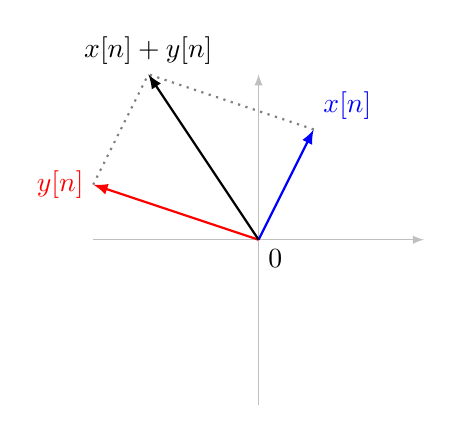
\begin{tikzpicture}[scale=0.7]
\path coordinate (a) at (0,0)
      coordinate (b) at (1.0,2.0)
      coordinate (c) at (-3, 1);
      coordinate (d) at (-2, 3.0);
\draw[thin, gray!50!, -latex] (-3, 0) -- (3, 0);
\draw[thin, gray!50!, -latex] (0, -3) -- (0, 3);
\draw[thick,blue,-latex] (a) -> (b);
\draw[thick,red,-latex] (a) -> (c);
\draw[gray, thick , dotted] (1, 2) -- (-2, 3);
\draw[gray, thick , dotted] (-3, 1) -- (-2, 3);
\draw[thick, black, -latex] (0, 0) -- (-2, 3);
\node[below right] at (a){$0$}; 
\node[blue,above right] at (b){$x[n]$};
\node[red,left] at (c){$y[n]$};
\node[black,above] at (-2, 3) {$x[n] + y[n]$};
\end{tikzpicture}
\end{center}
\end{frame}

\begin{frame}[t]{Representing signals in terms of other signals}
\begin{itemize}
  \item We can represent signals as linear combinations of other signals.
  \[ y[n] = \alpha_1 x_1[n] + \alpha_2 x_2[n] + \ldots + \alpha_m x_m[n] \implies y[n] \leftrightarrow \lp \alpha_i \rp_{i=1}^m \]

  \item The appropriate choice for $\lc x_i[n] \rc_{i=1}^m$ can provide a different perspective about the signal $y[n]$, which might not be immedaitely obvious in $y[n]$. 

  \vspace{-0.2cm}
  \begin{center}
  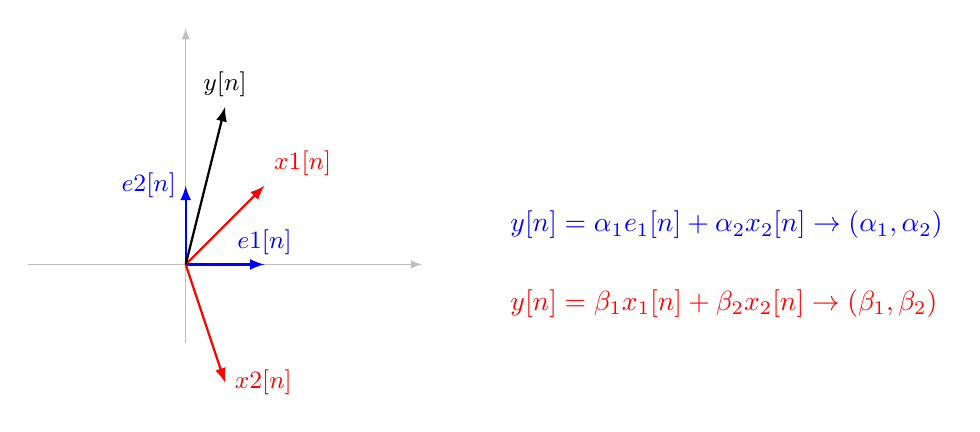
\begin{tikzpicture}[scale=1.0]
  \path coordinate (a) at (0,0)
        coordinate (e1) at (1, 0)
        coordinate (e2) at (0, 1)
        coordinate (x1) at (1, 1)
        coordinate (x2) at (0.5, -1.5)
        coordinate (y) at (0.5, 2.0);
  \draw[thin, gray!50!, -latex] (-2, 0) -- (3, 0);
  \draw[thin, gray!50!, -latex] (0, -1) -- (0, 3);
  \draw[thick, blue, -latex] (a) -> (e1);
  \draw[thick, blue, -latex] (a) -> (e2);
  \node[blue, above] at (e1) {\small $e1[n]$}; 
  \node[blue, left] at (e2) {\small $e2[n]$};
  \draw[thick, red, -latex] (a) -> (x1);
  \draw[thick, red, -latex] (a) -> (x2);
  \node[red, above right] at (x1) {\small $x1[n]$}; 
  \node[red, right] at (x2) {\small $x2[n]$};
  \draw[thick, black, -latex] (a) -> (y);
  \node[black, above] at (y) {\small $y[n]$}; 

  \node[blue, right] at (4, 0.5) {$y[n] = \alpha_1 e_1[n] + \alpha_2 x_2[n] \rightarrow \lp \alpha_1, \alpha_2 \rp$ };
  \node[red, right] at (4, -0.5) {$y[n] = \beta_1 x_1[n] + \beta_2 x_2[n] \rightarrow \lp \beta_1, \beta_2 \rp$ };
  \end{tikzpicture}
  \end{center}
\end{itemize}
\end{frame}

% % WHAT IS A SIGNAL?
% \begin{frame}{What is a signal? (Contd ... )}

% \begin{figure}
% 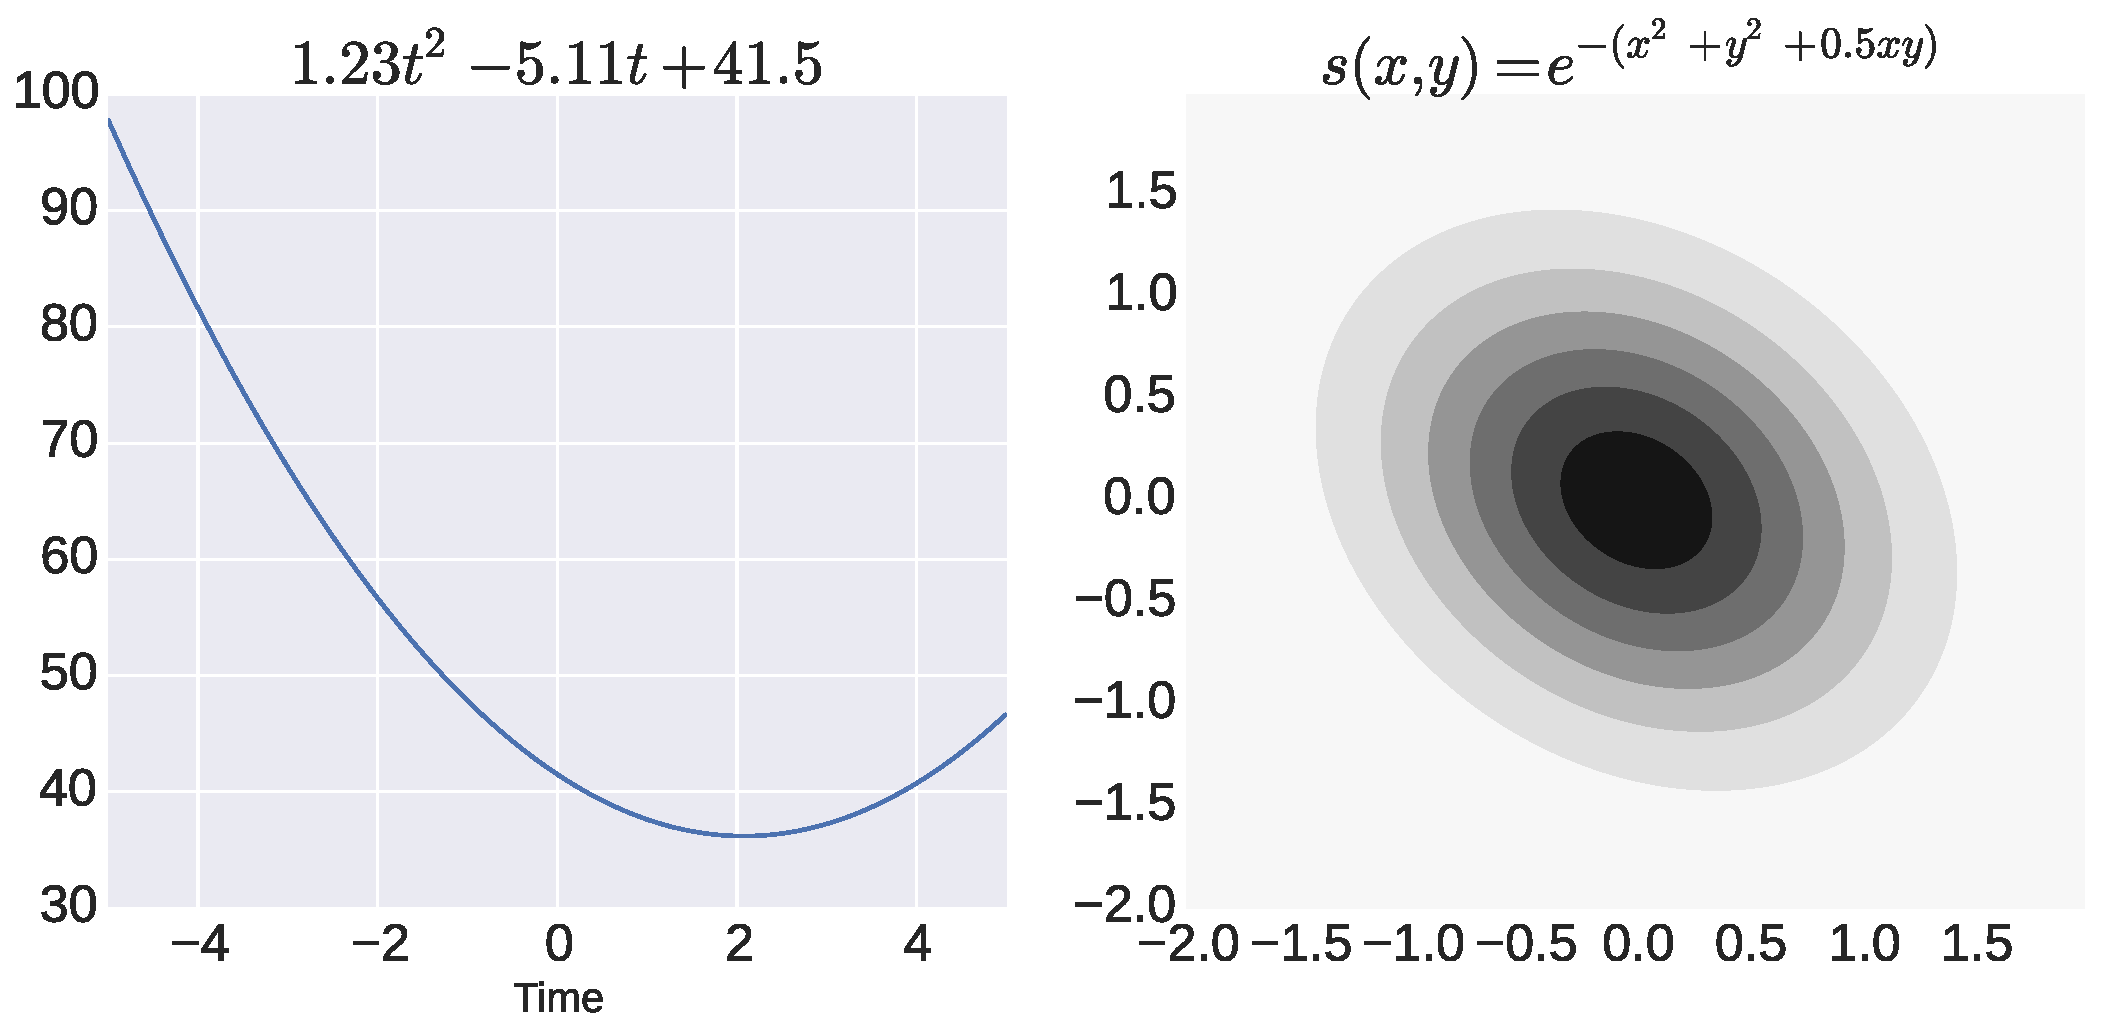
\includegraphics[width=0.7\textwidth]{img/signals.eps}
% \caption{Example of 1D and 2D signals}
% \end{figure}

% \textit{Can you think of examples of 3D and 4D signals?}
% \end{frame}

% \begin{frame}[t]
% \end{frame}

% % CLASSIFICATION OF SIGNALS
% \begin{frame}{Classification of signals}\
% \begin{itemize}
% \item Based on the signal dimensions. \textit{e.g.} 1D, 2D ...
% \item \textbf{Scalar} vs. \textbf{Vector} signals: \textit{e.g. gray scale versus RGB image}
% \[I_g\left(x,y\right) \in \mathbb{R} \,\,\mathrm{and}\,\, I_{color}\left(x,y\right) \in \mathbb{R}^3\]

% \end{itemize}
% \end{frame}


% \begin{frame}[t]
% \end{frame}


% % CLASSIFICATION OF SIGNALS
% \begin{frame}{Classification of signals}\
% \begin{itemize}
% \item \textbf{Continuous-time} vs. \textbf{Discrete-time}: \textit{based on the values assumed by the independent variable.}
% \[
% \begin{cases}
% x(t) = e^{-0.1t^{2}}, \,\, t \in \mathbb{R} & \text{Continuous-time} \\
% x[n] = e^{-0.1n^{2}}, \,\, n \in \mathbb{Z} & \text{Discrete-time}
% \end{cases}
%  \]
% \end{itemize}
% \begin{figure}
% 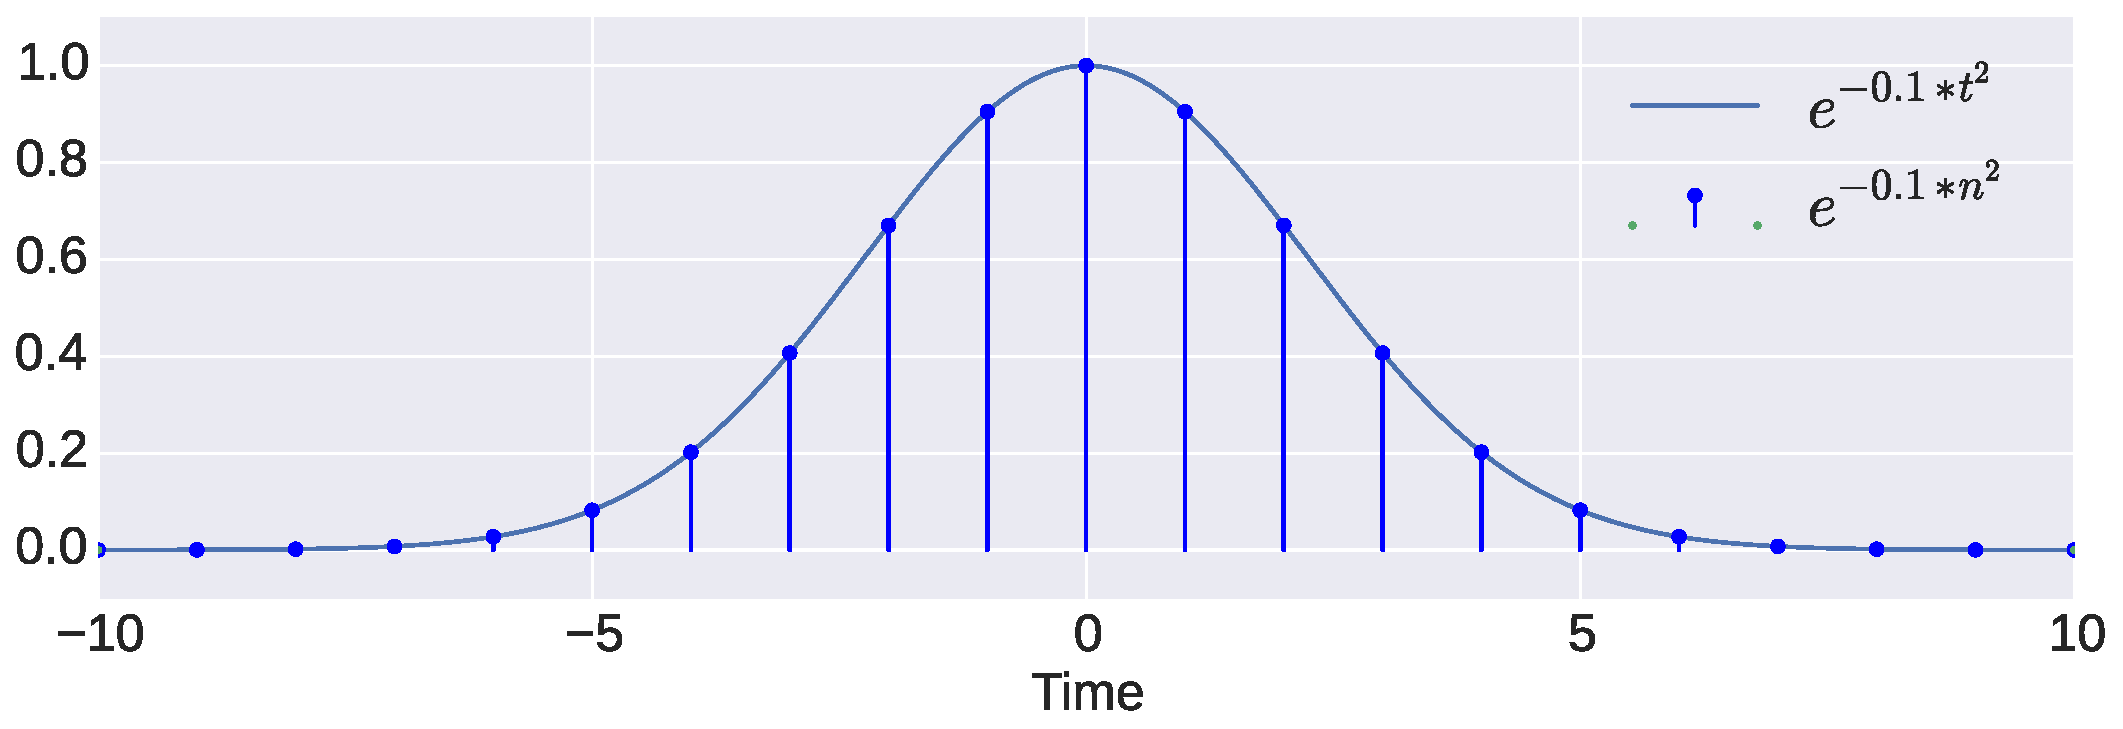
\includegraphics[width=0.7\textwidth]{img/cont_disc.eps}
% \end{figure}
% \end{frame}



% \begin{frame}[t]
% \end{frame}


% % CLASSIFICATION OF SIGNALS
% \begin{frame}{Classification of signals (Contd ...)}
% \begin{itemize}
% \item \textbf{Continuous-valued} vs. \textbf{Discrete-valued}: \textit{based on the values assumed by the dependent variable.}
% \[
% \begin{cases}
% x(t) \in [a, b] & \text{Continuous-valued} \\
% x(t) \in \{a_1, a_2, \ldots\} & \text{Discrete-valued} \\
% \end{cases}
%  \]
% \end{itemize}
% \begin{figure}
% 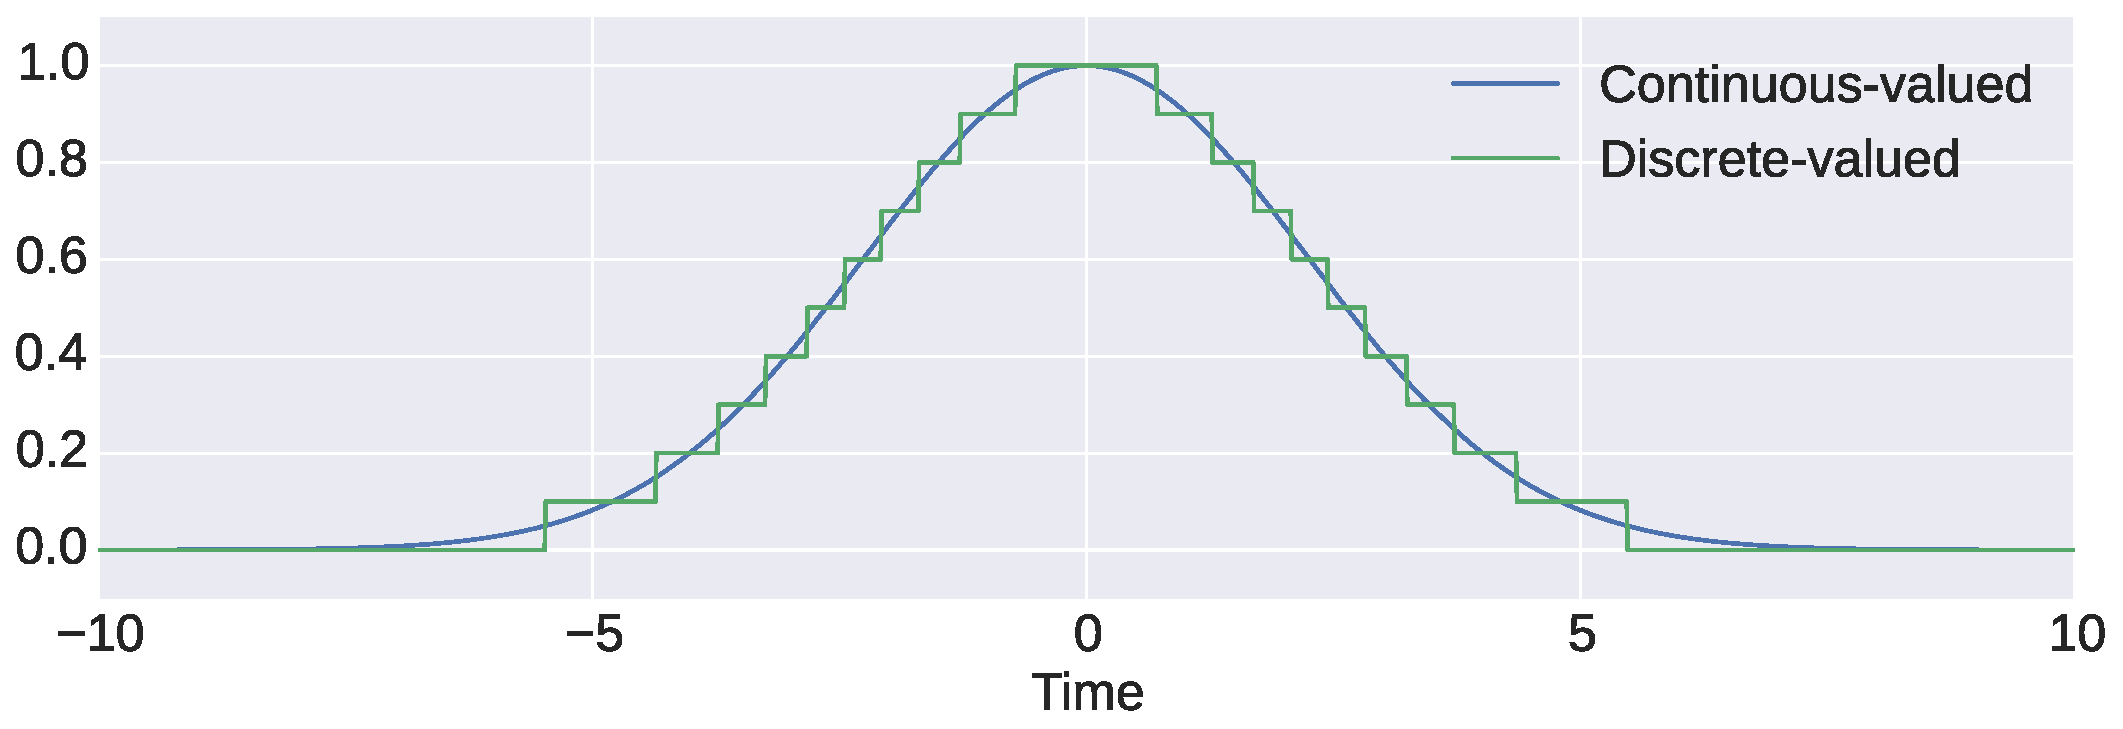
\includegraphics[width=0.7\textwidth]{img/cont_disc_val.eps}
% \end{figure}
% \end{frame}




% \begin{frame}[t]
% \end{frame}


% % CLASSIFICATION OF SIGNALS
% \begin{frame}{Classification of signals (Contd ...)}
% \textbf{Four types of signals}
% \begin{figure}
% 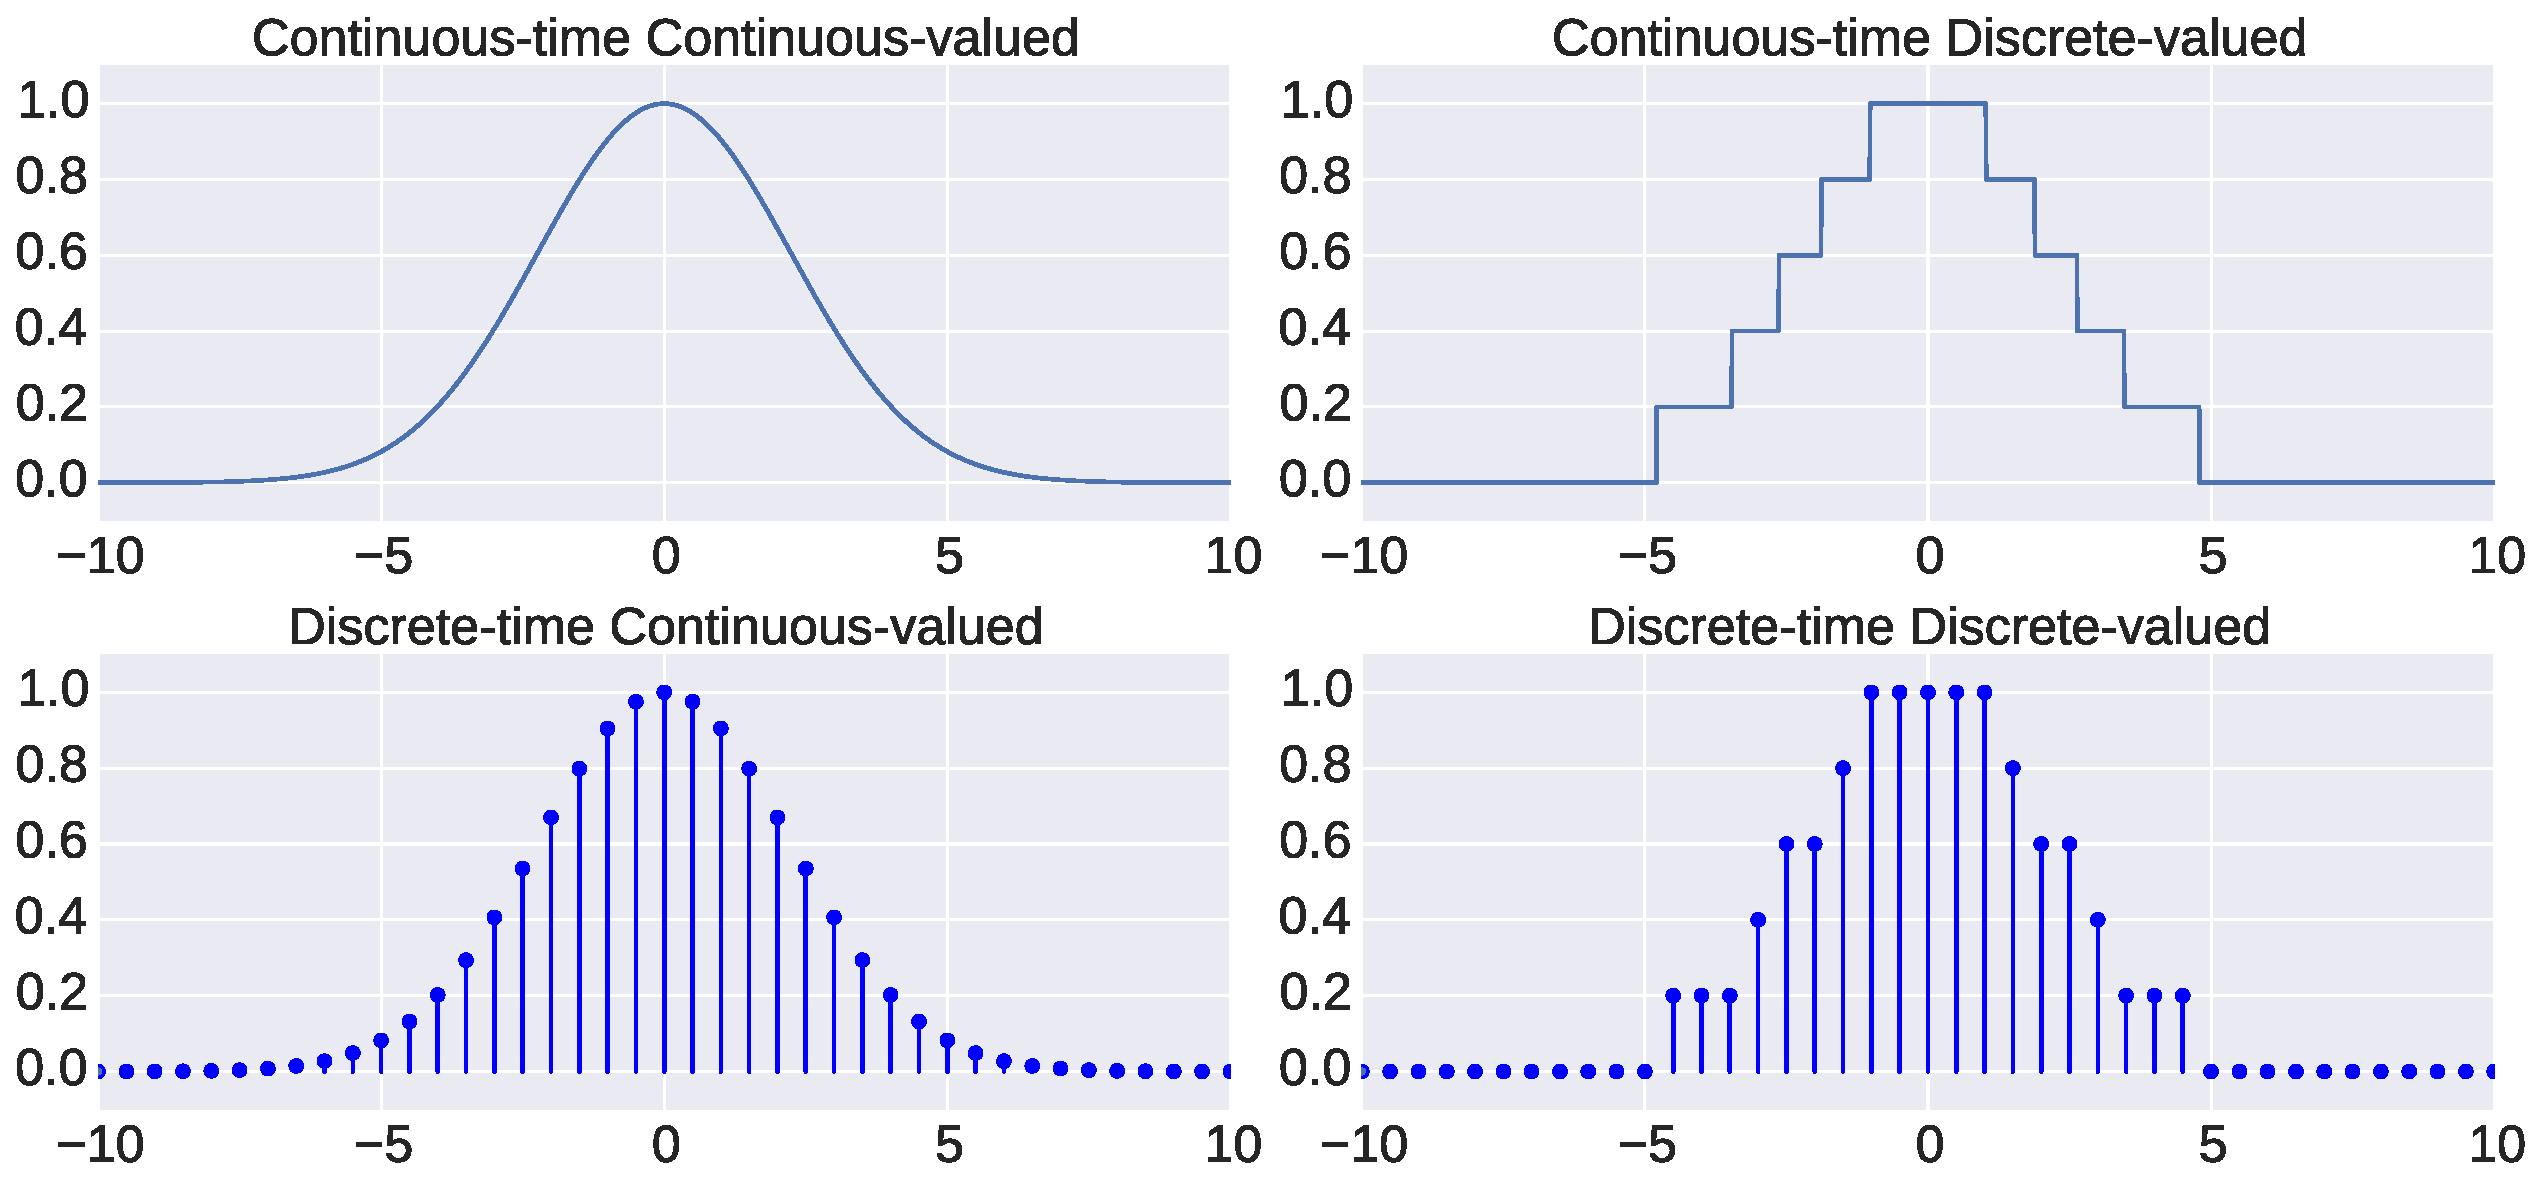
\includegraphics[width=0.8\textwidth]{img/signal_types.eps}
% \end{figure}
% \end{frame}


% \begin{frame}[t]
% \end{frame}


% % CLASSIFICATION OF SIGNALS
% \begin{frame}{Classification of signals (Contd ...)}
% \begin{itemize}
% \item \textbf{Deterministic} vs. \textbf{Stochastic}: \textit{e.g. EMG is an example of a stochastic signal.}
% \end{itemize}
% \begin{figure}
% 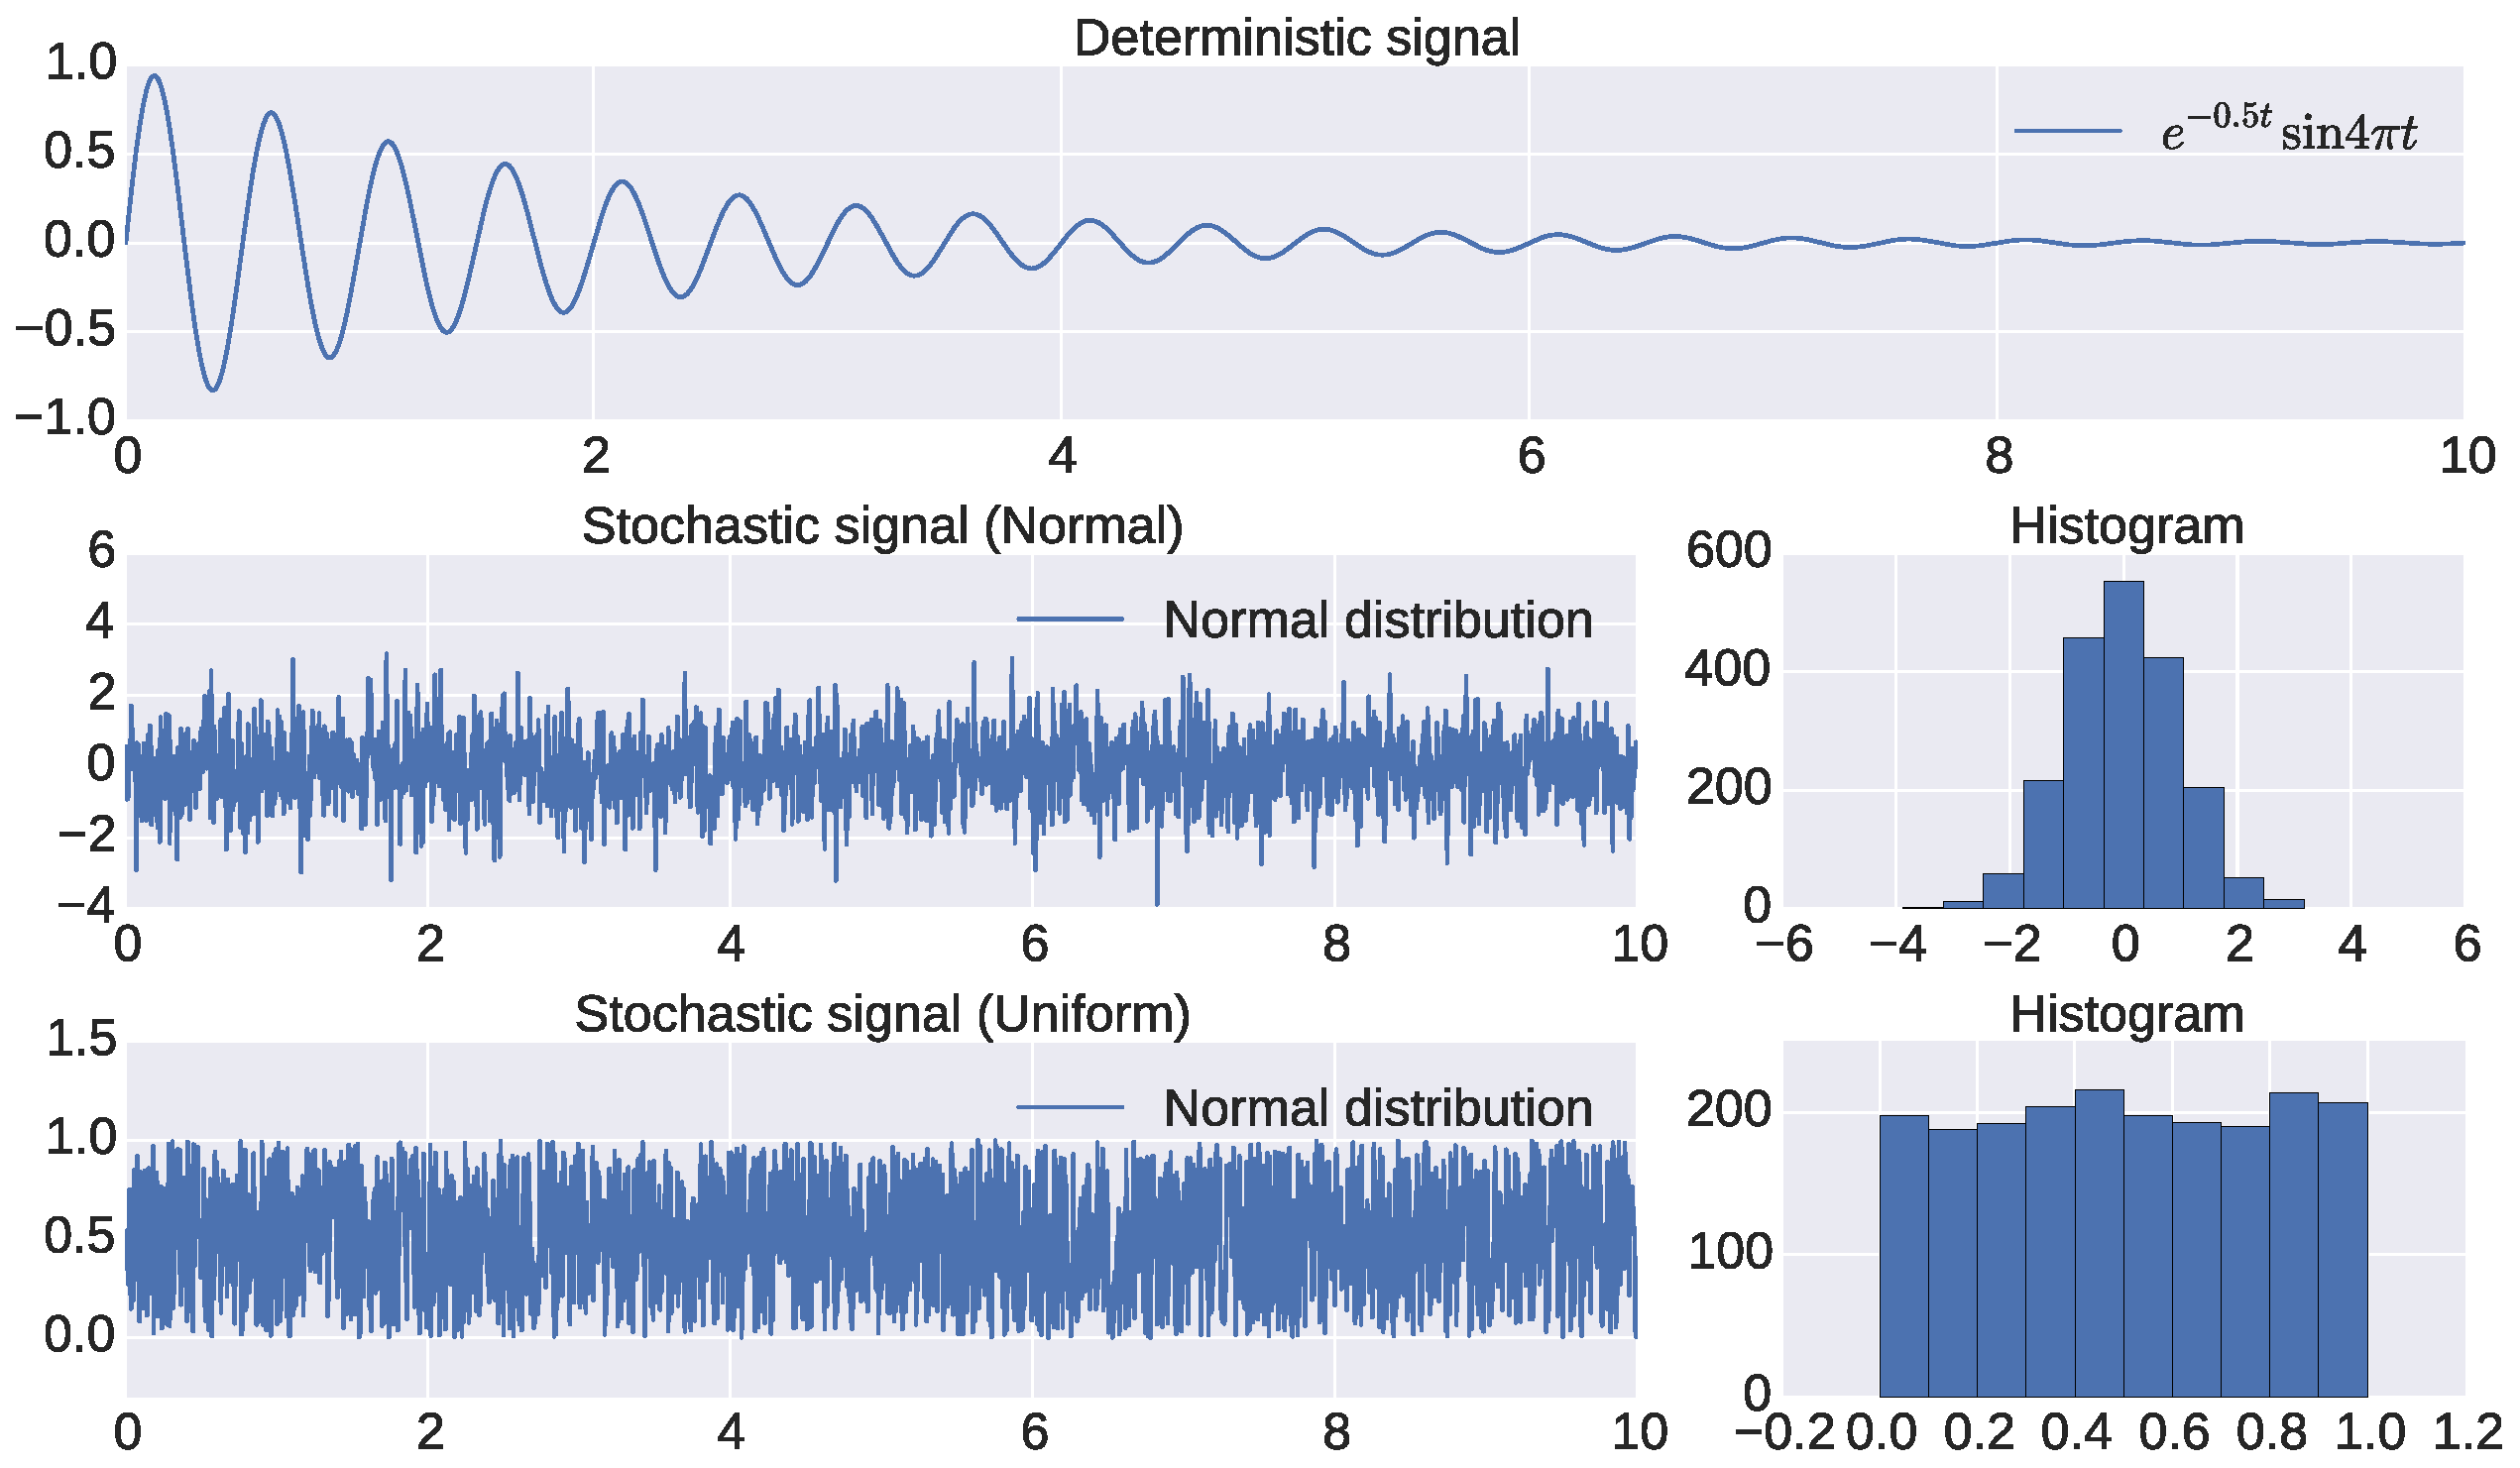
\includegraphics[width=0.75\textwidth]{img/det_stoch.eps}
% \end{figure}
% \end{frame}

% % CLASSIFICATION OF SIGNALS
% \begin{frame}{Classification of signals (Contd ...)}
% \begin{itemize}
% \item \textbf{Even} vs. \textbf{Odd}: \textit{based on the symmetry about the} $t=0$ \textit{axis}.
% \[\begin{cases}
% x(t) = x(-t), & \text{Even signal} \\
% x(t) = -x(-t), & \text{Odd signal} \\
% \end{cases}\]

% \textit{Most signals are neither even or odd?}

% \begin{tcolorbox}[width=0.9\textwidth,colback={lightgray},title={\textbf{Theorem}},colbacktitle=black,coltitle=white]
% \textit{Any arbitrary function can be represented as a sum of an odd and even function.}
% \[ x(t) = x_{even}(t) + x_{odd}(t) \]
% where, $ x_{even}(t) = \frac{x(t) + x(-t)}{2} $ and $ x_{odd}(t) = \frac{x(t) - x(-t)}{2} $.
% \end{tcolorbox}
% \end{itemize}
% \end{frame}

% % CLASSIFICATION OF SIGNALS
% \begin{frame}[t]{Classification of signals (Contd ...)}
% \textbf{Decomposition of an arbitrary signal into even and odd components}
% \begin{figure}
% 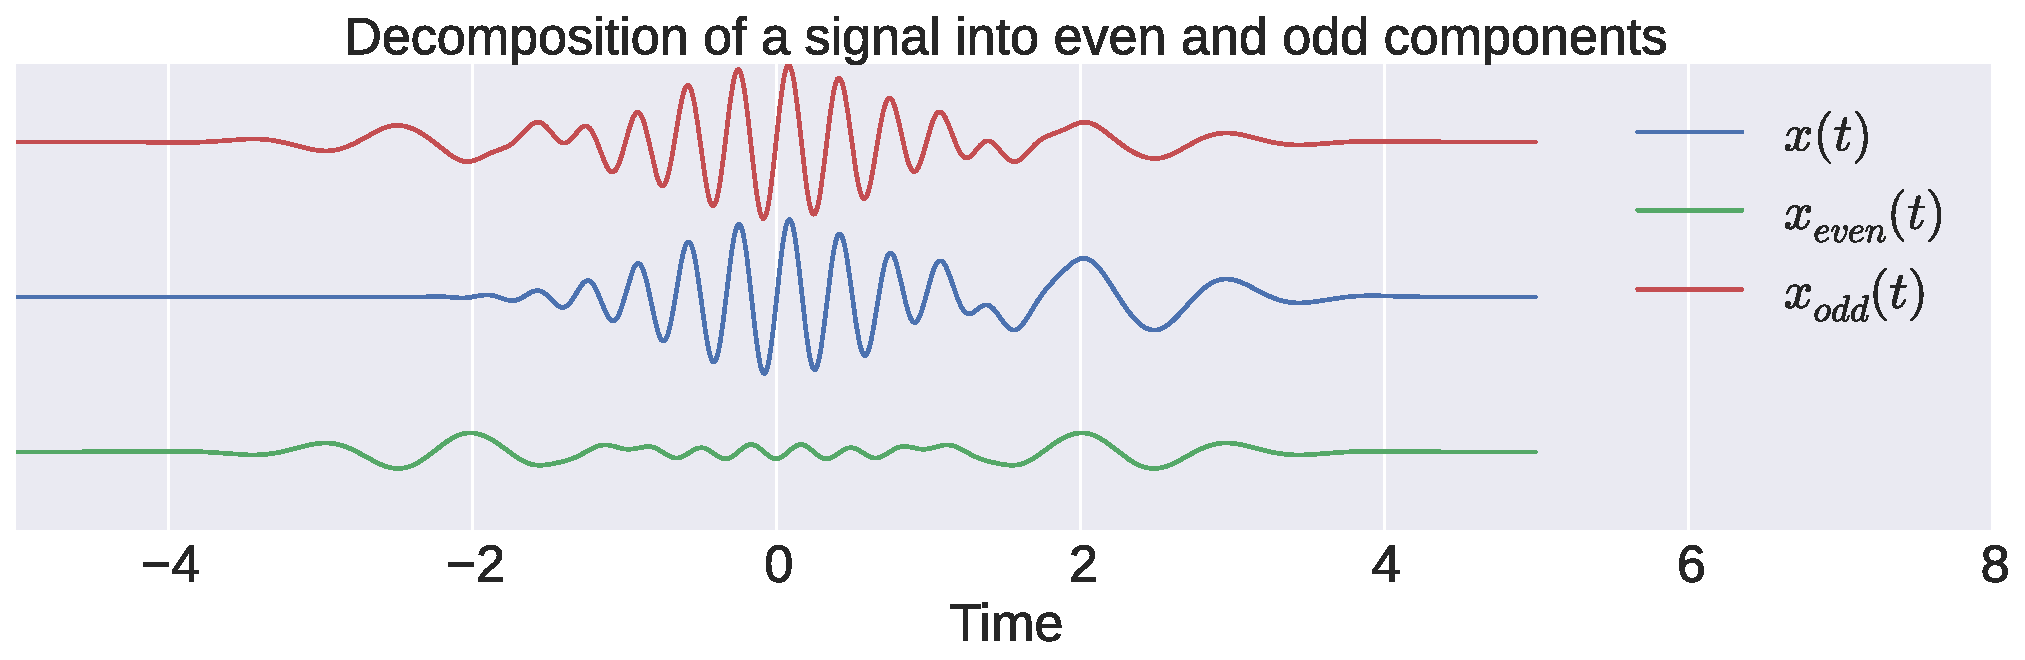
\includegraphics[width=\textwidth]{img/even_odd.eps}
% \end{figure}
% \end{frame}

% % CLASSIFICATION OF SIGNALS
% \begin{frame}[t]{Classification of signals (Contd ...)}
% \begin{itemize}
% \item \textbf{Periodic} vs. \textbf{Non-periodic}: \textit{a signal is periodic, if and only if}
% \[x\left(t\right) = x\left(t + T\right), \forall t\]
% where, $T$ is the fundamental period.
% \end{itemize}
% \end{frame}



% \begin{frame}[t]
% \end{frame}



% \begin{frame}[t]
% \end{frame}




% % % CLASSIFICATION OF SIGNALS
% % \begin{frame}[t]{Classification of signals (Contd ...)}
% % \begin{itemize}
% % \item \textbf{Energy} vs. \textbf{Power}: \textit{indicates if a signal is short-lived.}

% % % \[ E = \int_{-\infty}^{\infty}\left|x(t)\right|^2dt \,\,\,\,\,\,\,\,\,\, P=\frac{1}{T}\int_{-T/2}^{T/2}\left|x(t)\right|^2dt \]

% % \[ E = \sum_{-\infty}^{\infty}\left|x(t)\right|^2 \,\,\,\,\,\,\,\,\,\, P=\lim _{N \to \infty}\frac{1}{2N+1}\sum_{-N}^{N}\left|x(t)\right|^2 \]

% % \textit{A signal is an \textbf{energy} signal, if} $0 < E < \infty$.

% % \textit{A signal is an \textbf{power} signal, if} $0 < P < \infty$.
% % \end{itemize}
% % \end{frame}




% % \begin{frame}[t]
% % \end{frame}


% % USEFUL SIGNALS IN CONTINUOUS AND DISCRETE TIME
% \begin{frame}{Useful signals in continuous and discrete-time}

% We will look at some important signals, that we will often come across and are useful in the analysis of signals and systems.
% \begin{itemize}
% \item Exponential signals
% \item (Complex) Sinusoids
% \item Exponential sinusoids
% \item Impulse/Dirac delta function
% \item Step function
% \end{itemize}

% There are some important differences between the corresponding continuous and discrete-time signals.

% \end{frame}


% % REAL EXPONENTIALS
% \begin{frame}{Real Exponentials}

% \textbf{Continuous-time} version
% \[ x(t) = be^{at} \]

% where, $a, b, t \in \mathbb{R}$. $b$ is the amplitude and $a$ is the exponential growth or decay rate.

% \begin{figure}
% 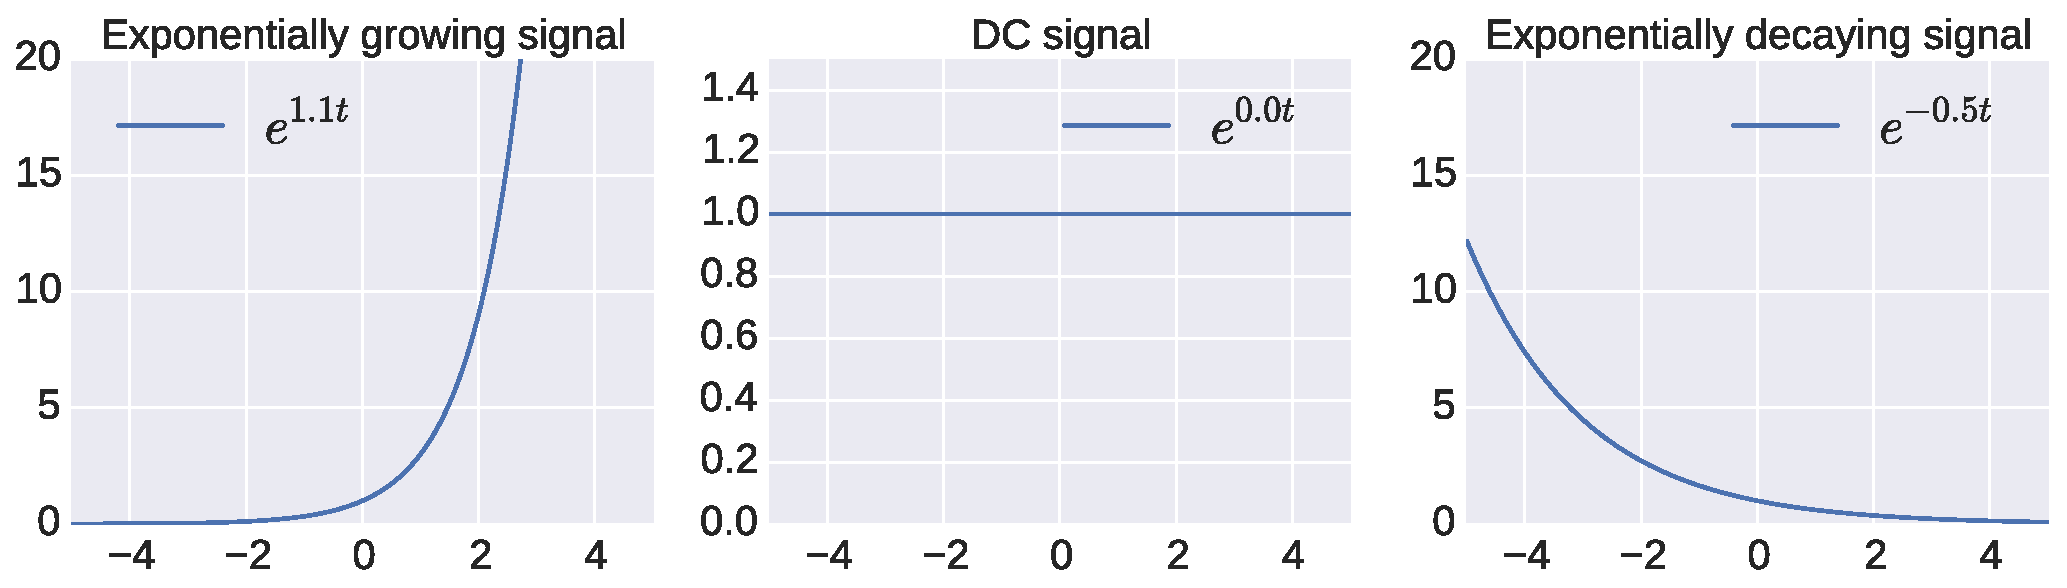
\includegraphics[width=\textwidth]{img/exp.eps}
% \end{figure}
% \end{frame}



% \begin{frame}[t]
% \end{frame}


% % REAL EXPONENTIALS
% \begin{frame}{Real Exponentials (Contd ...)}

% \textbf{Discrete-time} version
% \[ x[n] =  b \left(a\right)^n \]

% where, $a, b \in \mathbb{R}$ and $n \in \mathbb{Z}$. $b$ is the amplitude and $a$ is the exponential growth or decay rate.

% \begin{figure}
% 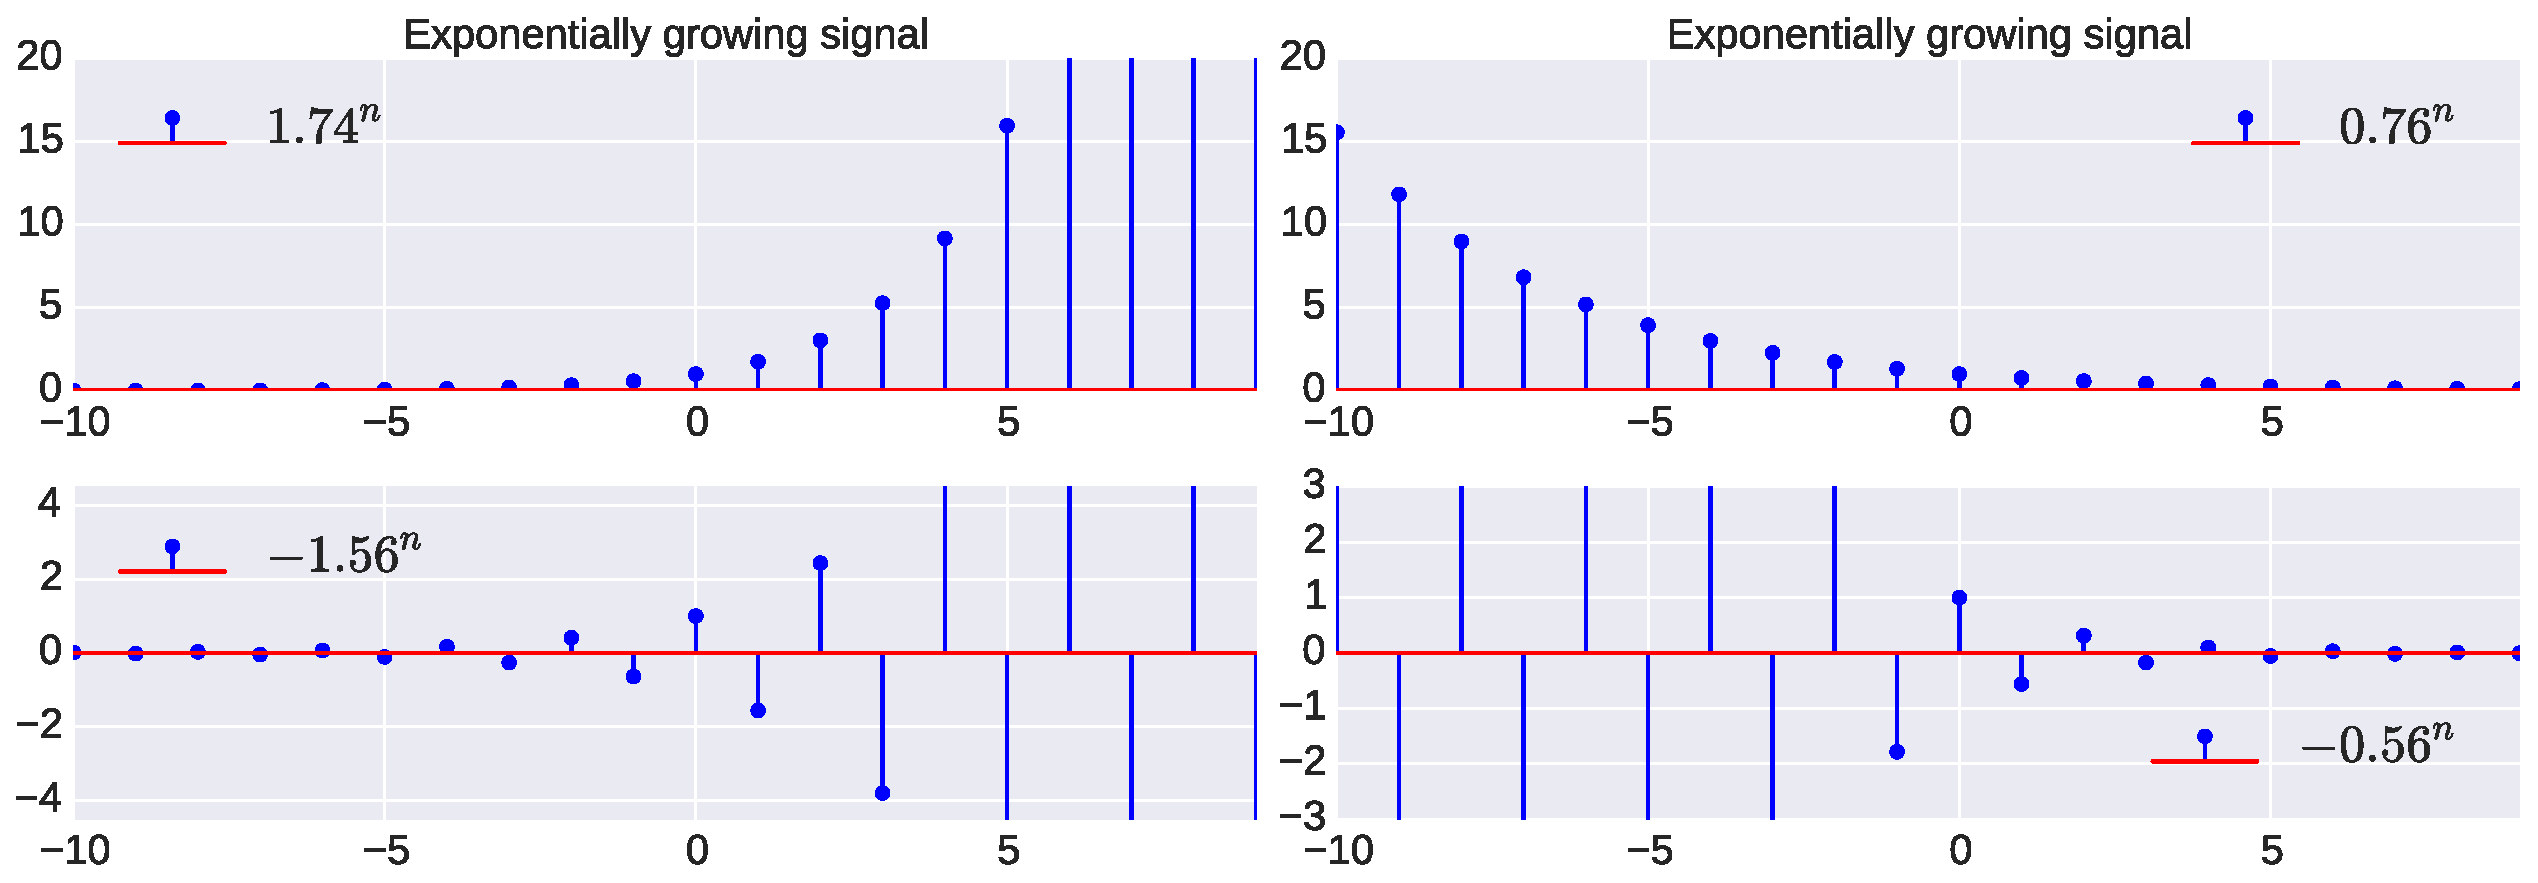
\includegraphics[width=\textwidth]{img/disc_exp.eps}
% \end{figure}
% \end{frame}



% \begin{frame}[t]
% \end{frame}


% % REAL EXPONENTIALS
% \begin{frame}{Real Exponentials (Contd ...)}

% These are encountered as solution to first order differential and difference equations.
% \[ \frac{d}{dt}x(t) = kx(t) \implies x(t) = Ce^{kt} \]
% \[ x[n] = kx[n-1] \implies x(t) = C(k)^n \]

% Can you think of practical examples of systems that result in such signals?
% \end{frame}



% \begin{frame}[t]
% \end{frame}


% % SINUSOIDAL SIGNALS
% \begin{frame}{Sinusoidal signals}
% \textbf{Continuous-time} version

% \[ x(t) = A \sin \left(\omega t + \phi\right) \]

% where, $A$ is the amplitude, $\omega$ is the angular frequency $\left(\mathrm{rad}.\mathrm{sec}^{-1}\right)$, and $\phi$ is the phase angle.

% \begin{figure}
% 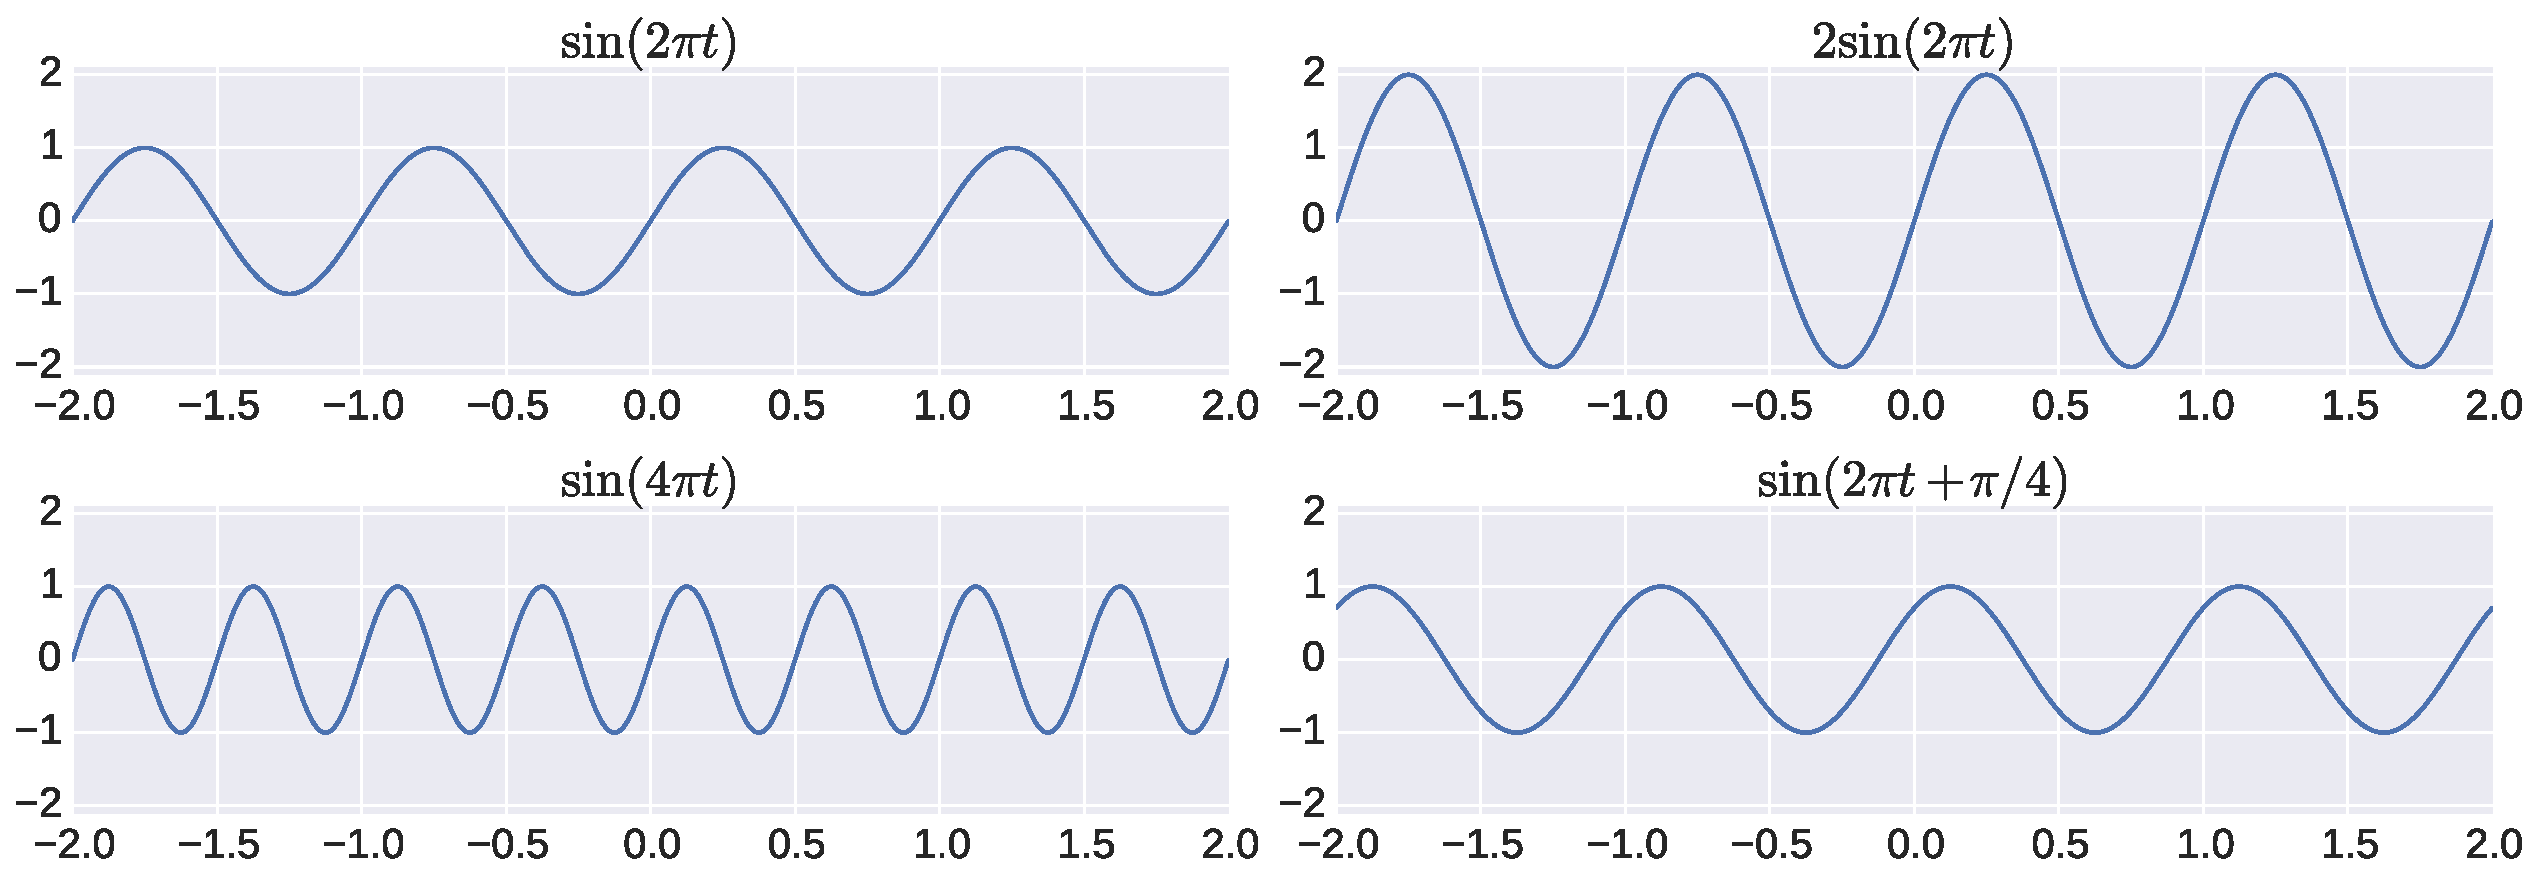
\includegraphics[width=0.8\textwidth]{img/sinu.eps}
% \end{figure}

% What is the fundamental period of sinusoid?
% \end{frame}



% \begin{frame}[t]
% \end{frame}



% \begin{frame}[t]
% \end{frame}



% \begin{frame}[t]
% \end{frame}



% % SINUSOIDAL SIGNALS
% \begin{frame}{Sinusoidal signals (Contd ...)}
% \textbf{Discrete-time} version

% \[ x[n] = A \sin \left(\Omega n + \phi\right) \]

% where, $A$ is the amplitude, $\Omega$ is the digital frequency $\left(\mathrm{rad}.\mathrm{sample}^{-1}\right)$, and $\phi$ is the phase angle.

% \begin{figure}
% 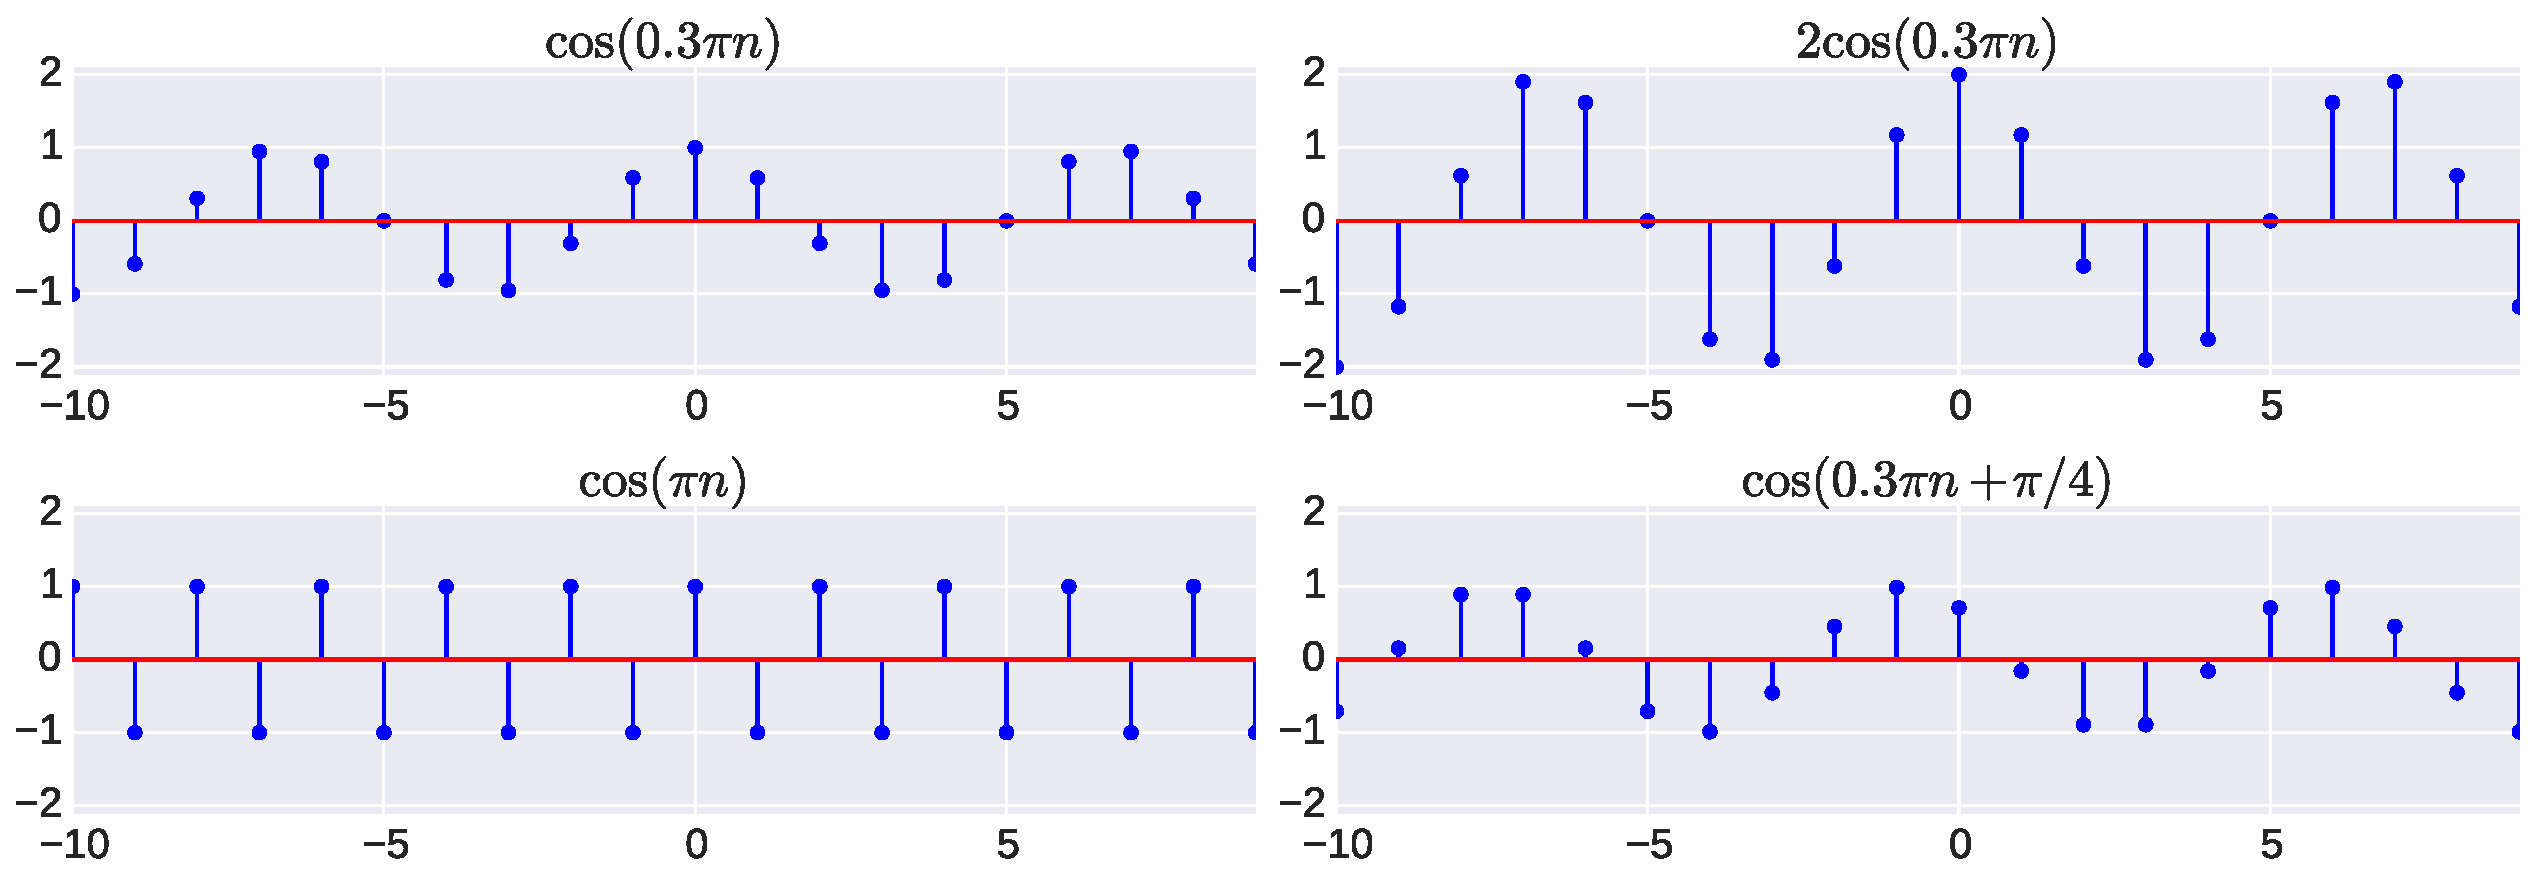
\includegraphics[width=0.8\textwidth]{img/disc_sinu.eps}
% \end{figure}

% What is the fundamental period?
% \end{frame}


% \begin{frame}[t]
% \end{frame}


% \begin{frame}[t]
% \end{frame}


% % SINUSOIDAL SIGNALS
% \begin{frame}{Sinusoidal signals (Contd ...)}

% \textbf{There are some peculiarities to the discrete sinusoid:}
% \begin{itemize}
% \item Not all sinusoids are periodic! e.g. $\sin(n)$
% \item There is a maximum frequency for discrete sinusoids. What is it?
% \item Two sinusoids that differ by a discrete frequency of $2\pi$ are the same sinusoids.
% \end{itemize}

% \end{frame}

% % SINUSOIDAL SINGALS
% \begin{frame}{Sinusoidal signals (Contd ...)}\

% \textbf{Complex exponential representation of sinusoids}

% \[ z = a + jb = \left|z\right|e^{j\theta} = \left|z\right|\cos \theta + j \left|z\right|\sin \theta\]

% \begin{figure}
% 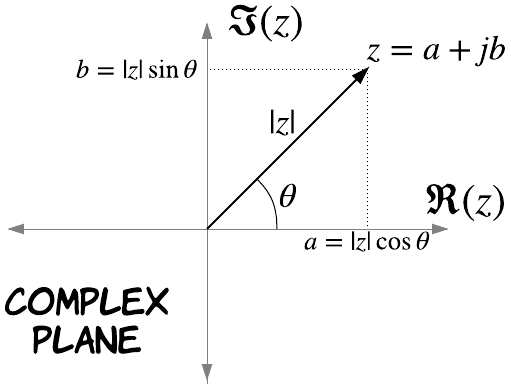
\includegraphics[width=0.5\textwidth]{img/complex_plane.png}
% \end{figure}

% \[ \cos \theta = \frac{e^{j\theta} + e^{-j\theta}}{2} \,\,\,\,\, \sin \theta = \frac{e^{j\theta} - e^{-j\theta}}{2j}\]

% \end{frame}


% \begin{frame}[t]
% \end{frame}


% \begin{frame}[t]
% \end{frame}


% % EXPONENTIAL SINUSOIDS
% \begin{frame}{Exponential sinusoids}
% \textbf{Continuous-time} version

% Amplitude modulated sinusoids
% \[ x(t) = a e^{bt} \sin \left(\omega t + \phi \right), \,\,\,\,\, a, b, \omega, \phi \in \mathbb{R}\]

% \begin{figure}
% 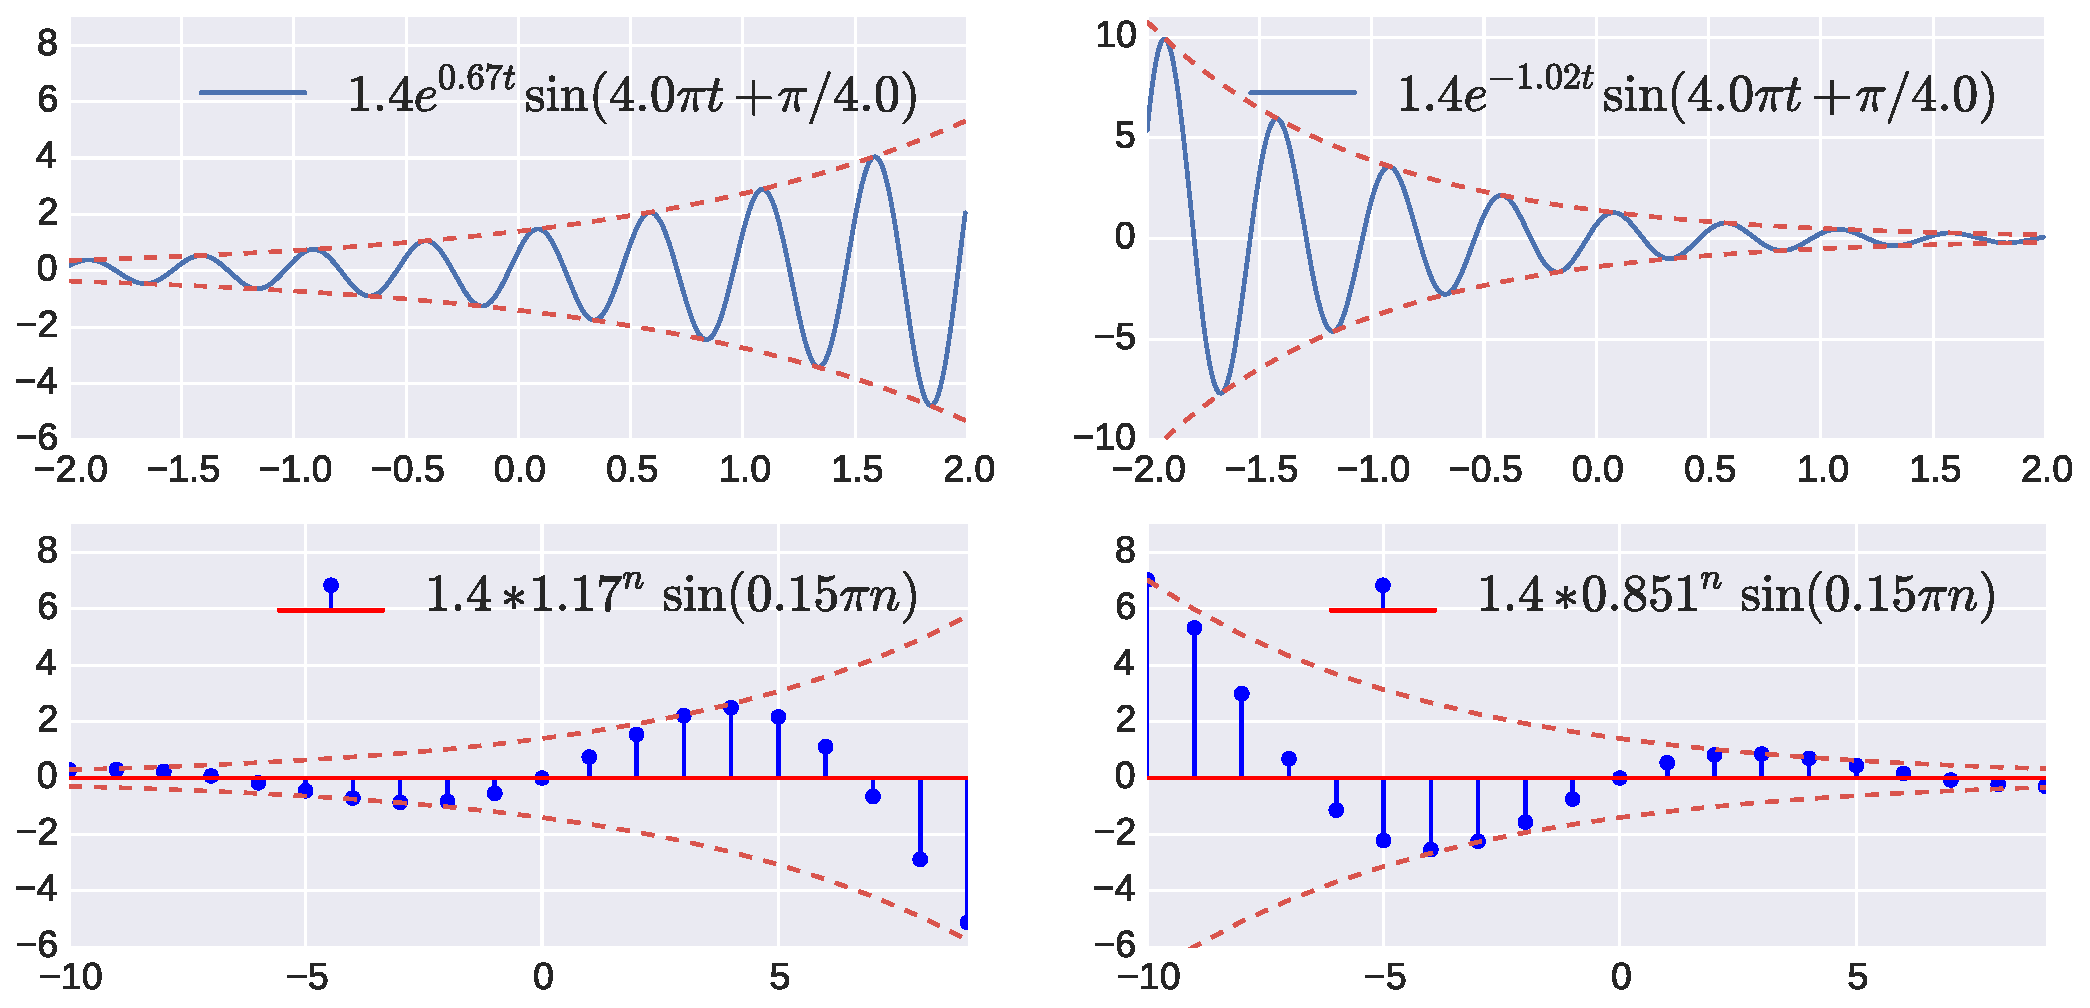
\includegraphics[width=0.8\textwidth]{img/exp_sin.eps}
% \end{figure}

% \end{frame}

% % % IMPULSE FUNCTION
% % \begin{frame}{Impulse function $\delta(t)$, $\delta[n]$}

% % \textbf{Dirac delta function} $\delta(t)$

% % \begin{itemize}
% % \item This is \textbf{\underline{NOT}} a conventional function.
% % \item It makes sense only when it is used in an integral.
% % \item It is not characterized by the exact values it takes as a function of the independent variable, but by the following important property.
% % \[ \int_{a}^{b}\delta (t) = \begin{cases}
% % 1, & 0 \in [a,b] \\
% % 0, & 0 \notin [a, b]
% % \end{cases} \]
% % \item It operates like a value selector.
% % \[ \int_{-\infty}^{\infty}f(t)\delta (t) = f(0), \text{, where $f$ is continuous at } t= 0. \]
% % \item Impulse function is a very useful theoretical tool for representing: point charges or masses, forces in instantaneous collisions, derivatives of jump discontinuities etc.
% % \end{itemize}
% % \end{frame}

% % % IMPULSE FUNCTION
% % \begin{frame}{Impulse function $\delta(t)$, $\delta[n]$ (Contd ...)}

% % $\delta(t)$ can be understood through a limiting operation. Let $f_{n}\left(t\right) = \begin{cases}
% % n, & -\frac{1}{2n} \leq t \leq \frac{1}{2n} \\
% % 0, & \mathrm{Otherwise}
% % \end{cases}$ and $\int_{-\infty}^{\infty}f_n(t)dt = 1$

% % \[\int_{-\infty}^{\infty}f_{n}\left(t\right)g\left(t\right)dt = \int_{-\frac{1}{2n}}^{\frac{1}{2n}}ng\left(t\right)dt = g_n \]

% % \[\lim_{n\to\infty}\int_{-\infty}^{\infty}f_{n}\left(t\right)g\left(t\right)dt = \lim_{n\to\infty}g_{n} = g\left(0\right) = \int_{-\infty}^{\infty}g(t)\delta(t)dt\]

% % \begin{figure}
% % 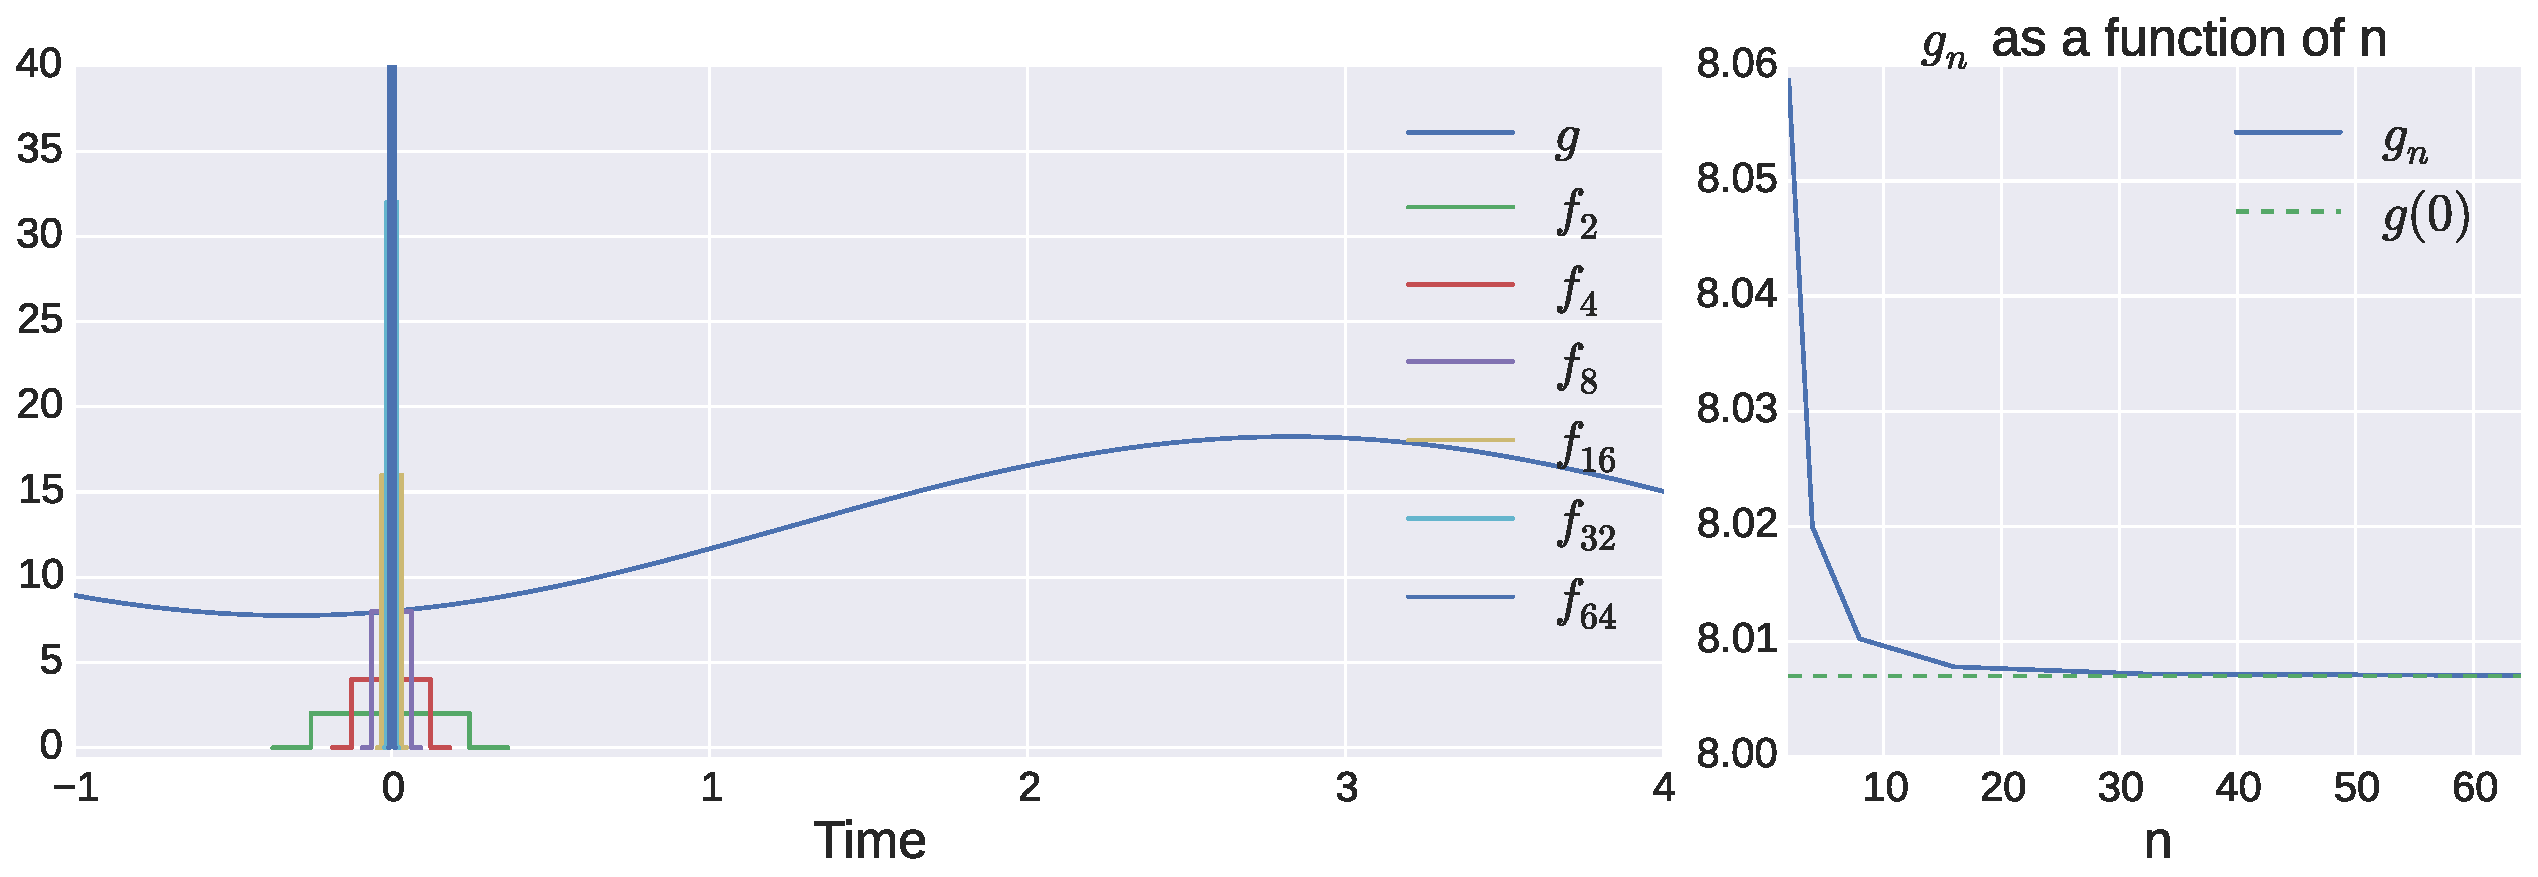
\includegraphics[width=\textwidth]{img/impulse_demo.eps}
% % \end{figure}
% % \end{frame}



% \begin{frame}[t]
% \end{frame}


% % IMPULSE FUNCTION
% \begin{frame}{Impulse function $\delta[n]$ (Contd ...)}

% \textbf{Kronecker delta function or sequence} $\delta[n]$

% \begin{itemize}
% \item \[ \delta[n] = \begin{cases}
% 1 & n = 0 \\
% 0 & \mathrm{Otherwise}
% \end{cases} \]
% \end{itemize}

% \begin{figure}
% 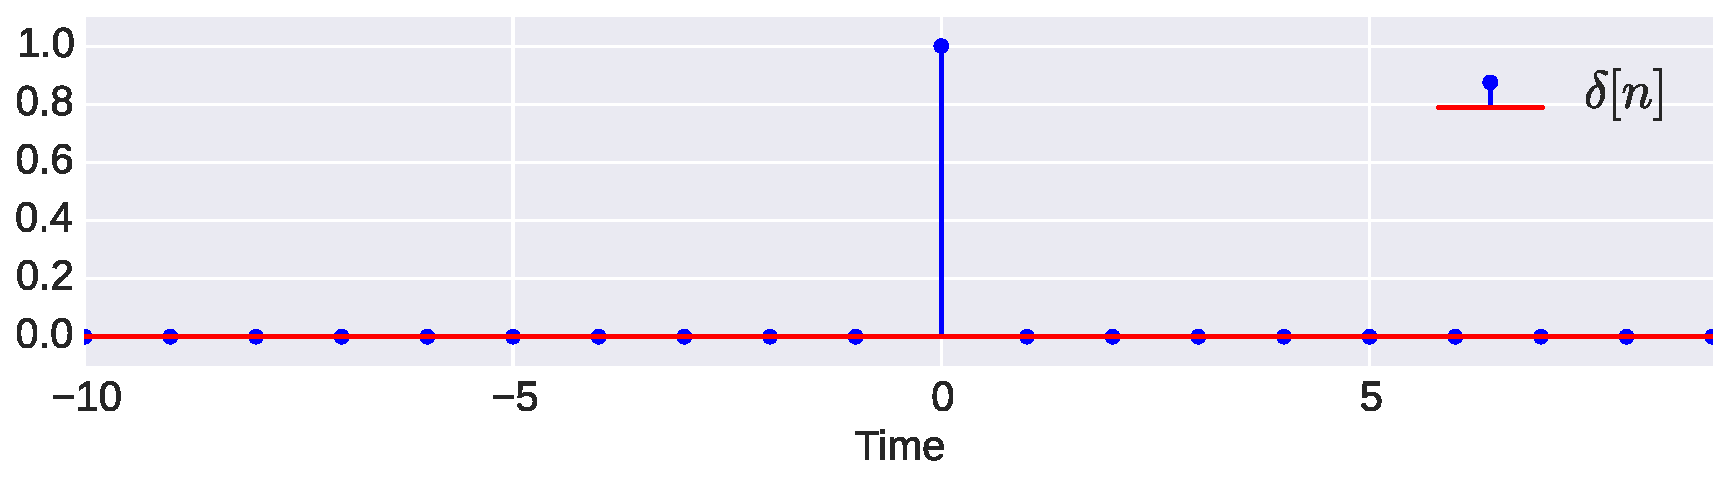
\includegraphics[width=\textwidth]{img/disc_imp.eps}
% \end{figure}
% \end{frame}



% \begin{frame}[t]
% \end{frame}


% % STEP FUNCTION
% \begin{frame}{Step function $u(t), u[n]$}

% \[ u[n] = \begin{cases} 1, & n \geq 0 \\ 0, & n < 0\end{cases} \]

% \begin{figure}
% 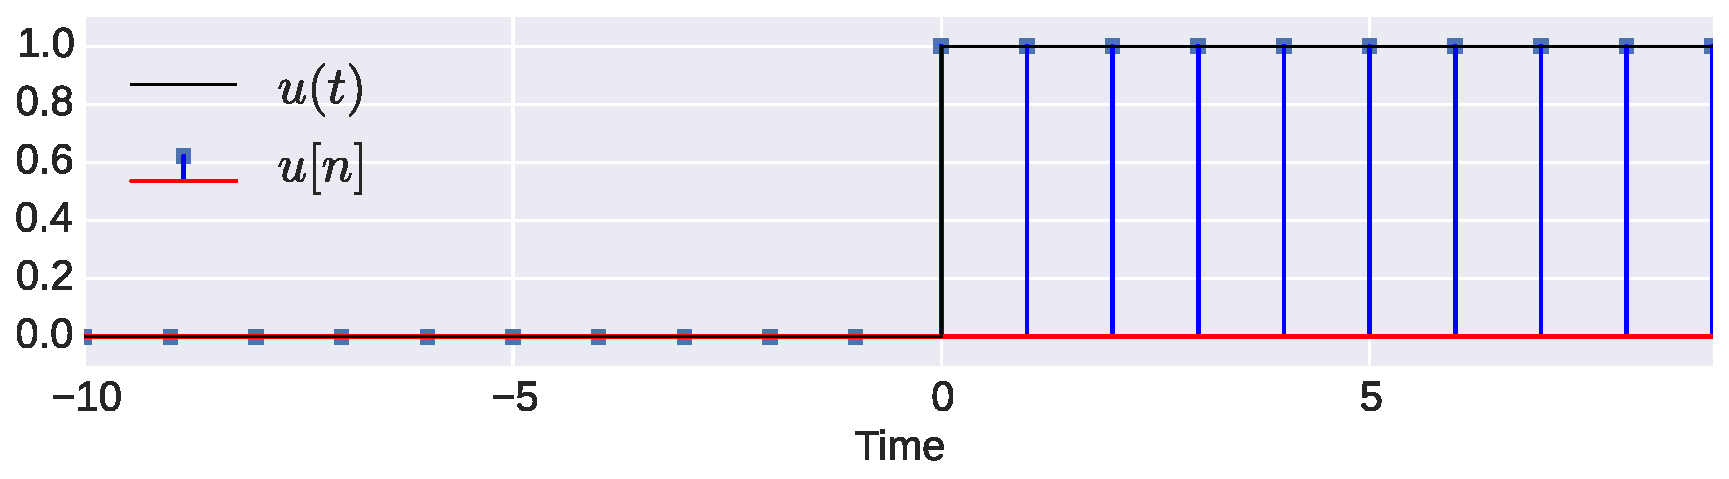
\includegraphics[width=\textwidth]{img/step.eps}
% \end{figure}

% \end{frame}



% \begin{frame}[t]
% \end{frame}




% % % WHAT IS A SYSTEM?
% % \begin{frame}{What is a system?}

% % A collection of objects united by some form of interaction or interdependence\footnote{Zadeh, Lotfi A., and Charles A. Deoser. \textit{Linear system theory}. New York: McGraw Hill, 1963.}.

% % \vspace{4mm}

% % From the signal processing point of view, \textbf{a system is any physical device or algorithm that performs some operation on a signal to transform it into another signal.}
% % B
% % \begin{figure}
% % 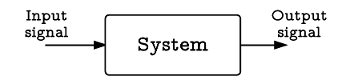
\includegraphics[width=0.7\textwidth]{img/system.png}
% % \end{figure}

% % Can be thought of a mapping function. \textit{e.g.}
% % \[ y = f\left(x\right) = kx \]

% % \end{frame}

% % % CLASSIFICATION OF SYSTEMS
% % \begin{frame}{Classification of systems}

% % Based on the properties of the system.

% % \begin{itemize}
% % \item \textbf{Linearity}: \textit{satisfies the properties of \textbf{scaling} and \textbf{superposition}}.

% % Let us assume, 
% % \[ f: x_i(t) \mapsto y_i(t) \]

% % The system $f$ is linear, if and only if,
% % \[ f:\sum_ia_ix_i(t) \mapsto \sum_ia_iy_i(t) \]

% % \textit{Which of these systems are linear?}
% % \begin{enumerate}
% % \item $y(t) = k_1x(t) + k_2x(t-2)$
% % \item $y(t) = \int_{t-T}^{t}x(\tau)d\tau$
% % \item $y(t) = 0.5x(t) + 1.5$
% % \end{enumerate}
% % \end{itemize}
% % \end{frame}

% % % CLASSIFICATION OF SYSTEMS
% % \begin{frame}{Classification of systems}

% % Based on the properties of the system.

% % \begin{itemize}
% % \item \textbf{Memory}: \textit{a system whose output depends on past or future values of its input is a system with memory, else the system is memoryless}. 

% % Note: the system may or may not depends on its present.

% % \[ \begin{cases}
% % y(t) = 0.5x(t) & \mathrm{\textbf{Memoryless system}} \\
% % y(t) = \int_{t-0.5}^{t}x(\tau)d\tau & \mathrm{\textbf{System with memory}}
% % \end{cases}
% % \]
% % \end{itemize}

% % \begin{figure}
% % 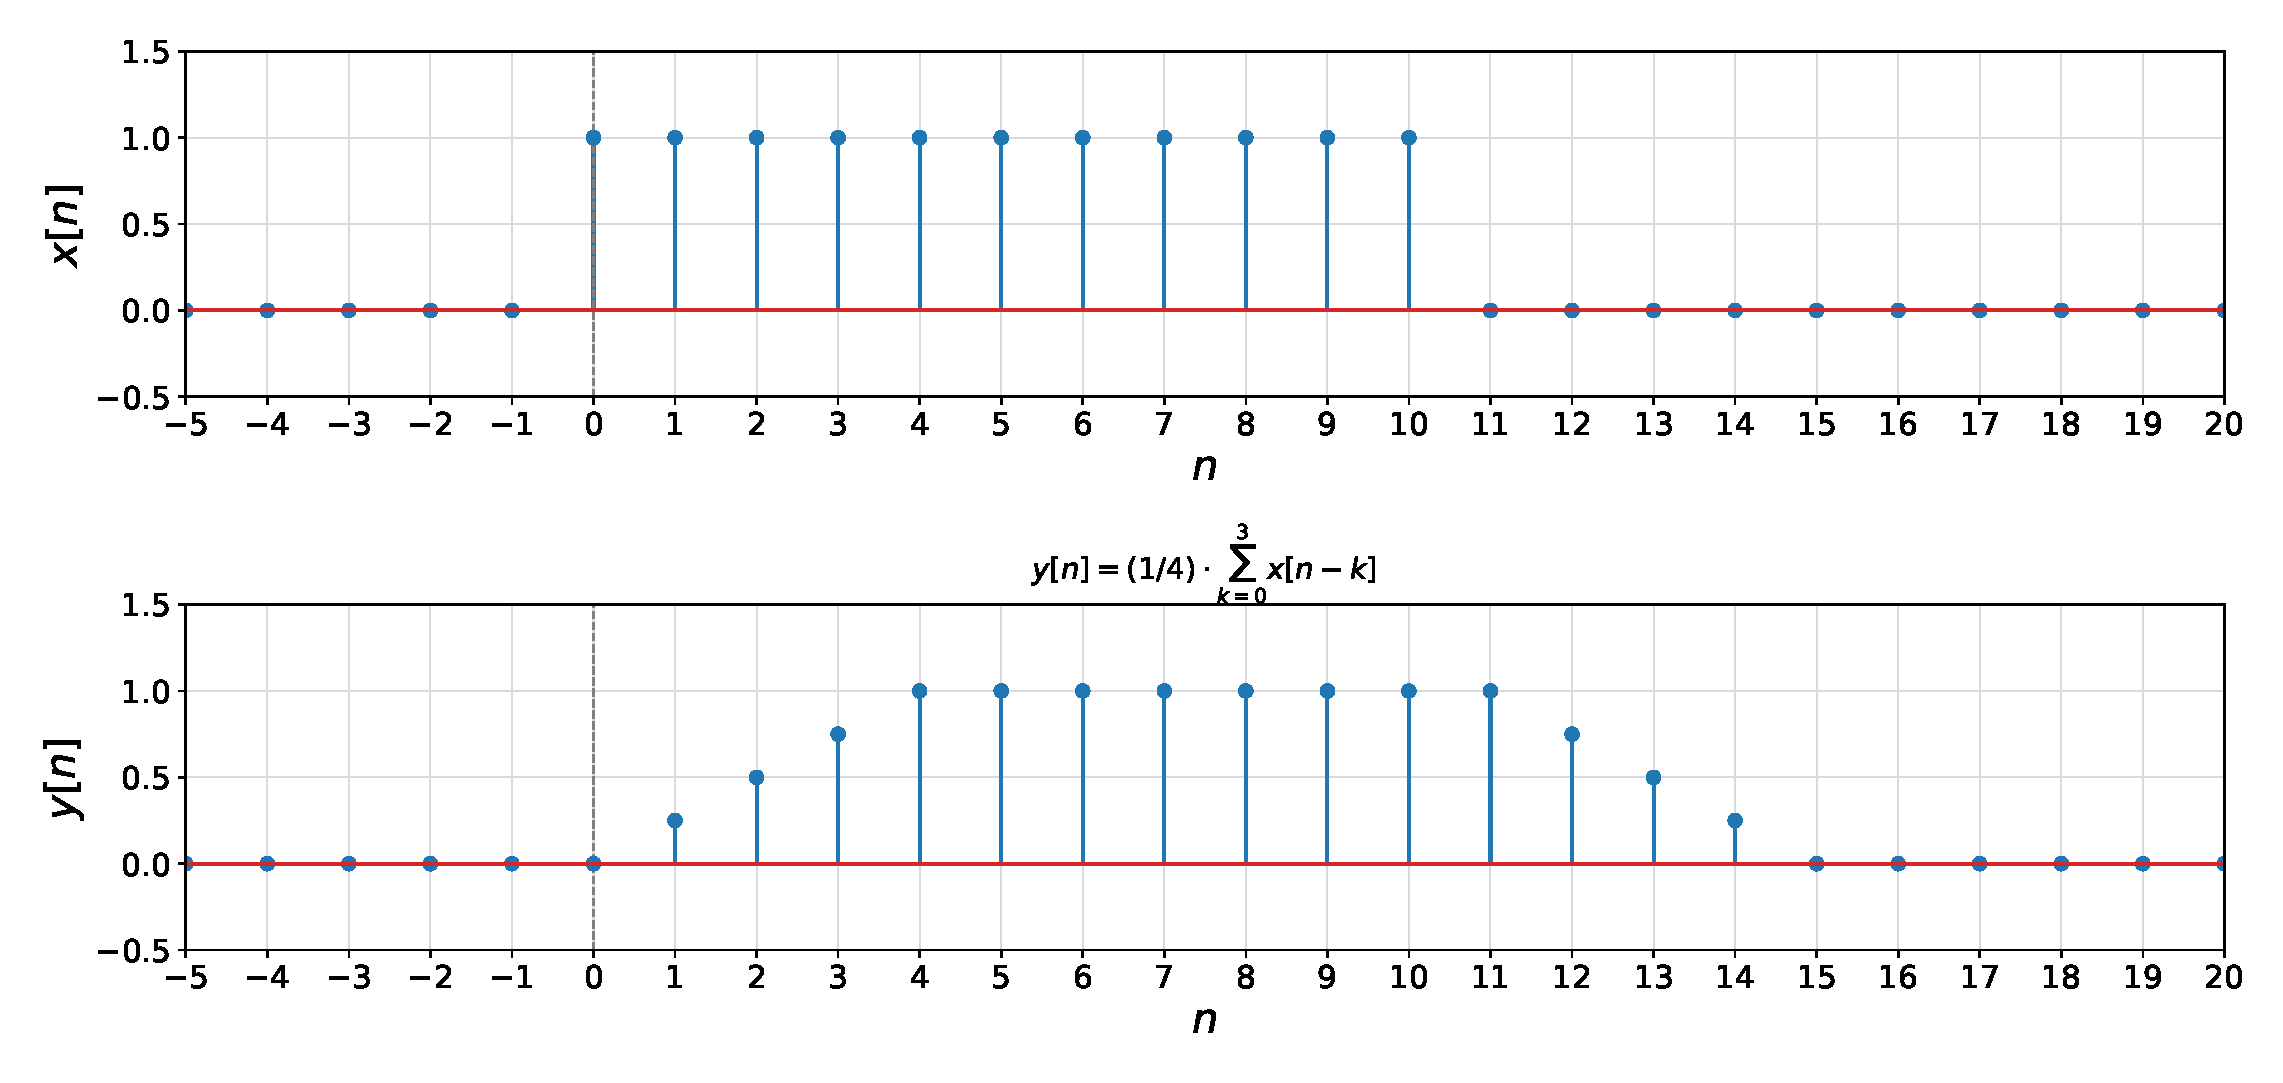
\includegraphics[width=0.7\textwidth]{img/memory.eps}
% % \end{figure}

% % \end{frame}

% % % CLASSIFICATION OF SYSTEMS
% % \begin{frame}{Classification of systems}

% % \begin{itemize}
% % \item \textbf{Causality}: \textit{a system whose output depends on the past and present only values of the input is a causal system}.
% % \[ \begin{cases}
% % y(t) = \int_{t-0.5}^{t}x(\tau)d\tau & \mathrm{\textbf{Causal}} \\
% % y(t) = \int_{t-0.5}^{t+0.5}x(\tau)d\tau & \mathrm{\textbf{Non-causal}}
% % \end{cases}
% % \]

% % \item \textbf{Time invariance}: \textit{system remains the same with time}.

% % If s system is time-invariant, then
% % \[ f:x\left(t\right) \mapsto y\left(t\right) \iff f:x\left(t-t_0\right) \mapsto y\left(t-t_0\right)\]

% % \item \textbf{Stability}: \textit{bounded input produces bounded output}.

% % \[ \left|x\left(t\right)\right| < M_x < \infty \mapsto \left|y\left(t\right)\right| < M_y < \infty \]

% % \item \textbf{Invertibility}: \textit{input can be recovered from output}.
% % \end{itemize}
% % \end{frame}

\end{document}